\documentclass{article} % \documentclass{} is the first command in any LaTeX code.  It is used to define what kind of document you are creating such as an article or a book, and begins the document preamble

\usepackage{amsmath, listings, graphicx, float, bbm, hyperref, amssymb, setspace, indentfirst, dcolumn, booktabs, url, changepage, tabularx, adjustbox, caption, amsthm, subcaption}
\usepackage[table]{xcolor}
\usepackage[normalem]{ulem}
\usepackage[authoryear, round]{natbib}
\usepackage[margin=1in]{geometry}
\setcitestyle{aysep={,},yysep={,},citesep={;},maxcitenames=2}

\title{Charter School Heterogeneity: CF Output Tables} % Sets article title
\author{Nicholas Lacoste} % Sets authors name
\date{\today} % Sets date for date compiled

% The preamble ends with the command \begin{document}
\begin{document} % All begin commands must be paired with an end command somewhere
    \maketitle % creates title using infromation in preamble (title, author, date)

I display the following figures and tables for each of the 3 main outcomes (Graduation rates, Math scores, ELA scores) in this order:
\begin{enumerate}
	\item \textbf{Variable Importance Factors (VIF)} -- These represent the depth-weigthed share of trees that split along a given covariate in the causal forest. Earlier splits are weighted more heavily. This produces a simple measure for the relative predictive power of each covariate in mapping heterogeneous treatment effects. For example, a VIF = 0.2 for variable $k$ would indicate that approximately 20\% of trees split on variable $k$. This is approximate because it may be that fewer than 20\% of the trees used variable $k$ if the trees that did use $k$ tended to split earlier on it, or more than 20\% if they tended to split later.
	\item \textbf{CATE Distribution} -- This is the distribution of district $\times$ year treatment effects. They're interpreted as average partial effects on a given district in a given year. For example, a coefficient of 0.5 indicates that increasing the charter share in district $d$ in year $t$ would have increased the outcome by 0.5pp.
	\item \textbf{Group Covariate Means} -- I display a table which examines the averages of each predictive covariate within districts that have significantly positive CATEs vs. districts that have significantly negative CATES. I also include the difference-in-means, though I have not yet added stars to highlight if the difference in statistically significant. 
	\item \textbf{ATE's of pre-specified subgroups (GATEs)} -- For now I just look at a few subgroups, but I plan to add more as we see fit. These tables display the average treatment effect within districts that meet a specified criteria. For example, I examine the group average treatment effect (GATE) for districts that are ``urban" vs. ``suburban" vs. ``rural." I also include (arbitrarily) the GATE of districts where $> 20\%$ of students are on free lunch.
	\item \textbf{Best Linear Projection (BLP)} -- Here I run a regression of each covariate on the predicted treatment effect: $\hat{\tau}(x) = \alpha + \boldsymbol{\beta} \boldsymbol{X}_i + \varepsilon$. The coefficients highlight the (linear) correlation between covariate values and the treatment effects. So for example, if the coefficient of log(enrollment) is positive, then this indicates that greater values of log(enrollment) are associated with larger CATE estimates. Note that I only use the top 5 covariates according to VIF score. 
\end{enumerate}

	Overview of results:
\begin{itemize}
	\item \underline{Treatment effect distributions:} The good news is that the ATE estimates are more-or-less similar to the ATE estimates from the original paper. The first thing to note, however, is that these are early results based on shallow forests (only 1,000 trees -- I would probably use around 10,000 in the final model) and that I perform global recentering which we know is not the correct approach (i.e. we need the local-recentering approach from the ``causal forest with fixed effects" algorithm). So, I suspect that this is causing some bias in the estimates of the ATE and the heterogeneous treatment effects. It also might be affecting precision, since we don't observe many statistically significant district $\times$ year CATE estimates.
	\item \underline{Important covariates:} We notice many of the same variables popping up with high VIF scores in each case.
	\begin{enumerate}
		\item ``Teacher salary" is in the top 3 VIF scores in each model, though it is only associated positively with higher test scores and not with graduation rates.
		\item ``log(enrollment)" is also a top variable. Greater enrollment tends to be associated positively with greater graduation rate and ELA scores, but negatively with math scores. 
		\item ``Percent black"  is a top 3 variable regarding test scores, but not with graduation rates. For both Math and ELA it is associated with lower test scores. 
		\item ``Student-teacher ratio" is in the top 4 in both Math and ELA, but not graduation rates. In both ELA and Math a higher S/T ratio seems to be slightly associated with positive test scores
	\end{enumerate}
	\item \underline{GATEs I looked at:} So far all I have checked as far as within-group ATEs are the Urban vs. Suburban vs. Rural, and if the district has a $> 20\%$ free lunch rate. Urban and Suburban districts tent to have (sometimes imprecisely) higher ATEs for graduation rates and Math scores, but Rural districts haev (fairly precisely) greater ATEs in ELA. ``$> 20\%$ Percent free lunch" is assocated positively with larger ATEs for both graduation rates and ELA, but not with Math. 
\end{itemize}

	Next steps:
\begin{itemize}
	\item Some more tables to make: (1) GATEs within states, (2) GATEs within more subgroups, (3) GATEs within different levels of the treatment dosage, (4) CATEs within districts (here I examine district $\times$ year treatment effects, we likely want to average over district).
	\item Need to make deeper forests and use CFFE. These are relatively shallow forests (only 1000 trees, which is fewer than probably needed for valid CI's), and I use global recentering which we know will yield biased estimates. So these results are merely a flavor of what the real results will be.
\end{itemize}

	\section{Graduation Rate Results}

\begin{figure}[H]
\centering
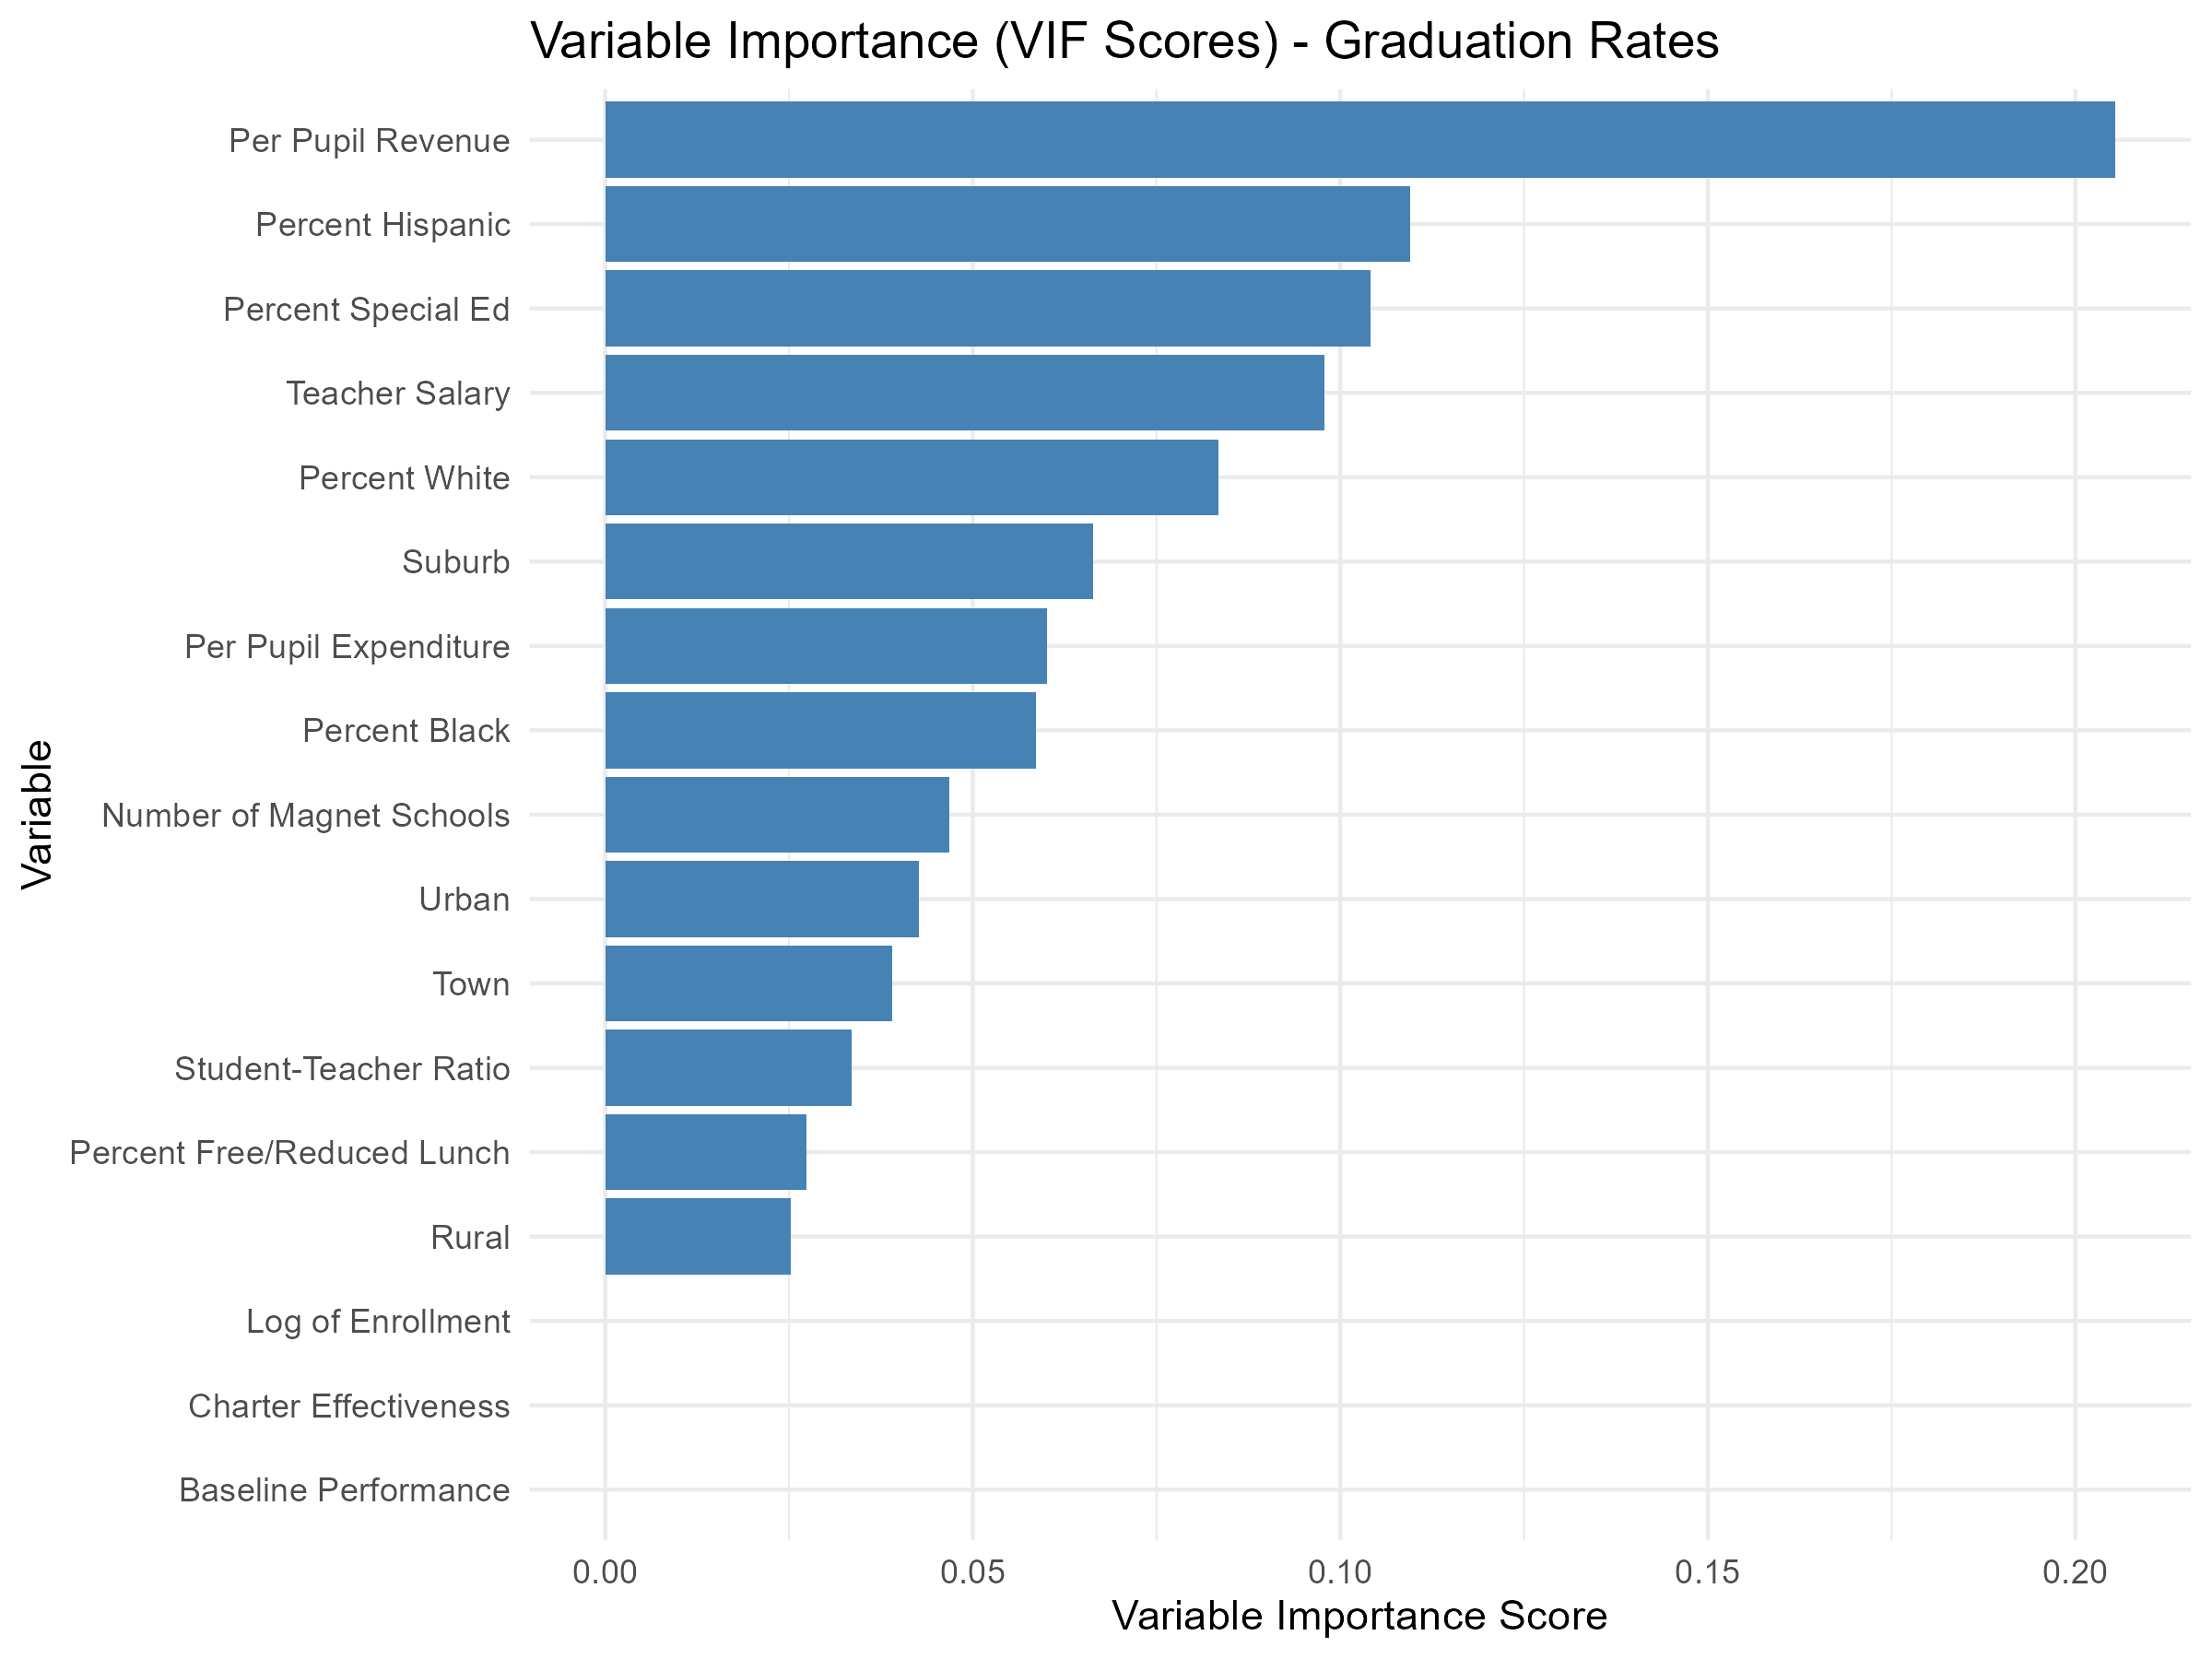
\includegraphics[width=\textwidth]{c:/Users/nickm/OneDrive/Acer (new laptop)/Documents/PhD/Tulane University/Projects/Charter School Heterogeneity/Charter_School_Heterogeneity_Project/analysis/output/figures/vif_scores_afgr.png}
\caption{VIF Scores: Graduation Rates}
\label{fig:image1}
\begin{minipage}{1\linewidth}
\singlespacing
\footnotesize
\emph{Notes}: Figure 1 plots VIF scores -- the share of total trees which use a given baseline covariate to perform splitting, weighted by the depth at which the split occurred so that earlier splits within a tree count for slightly more.  
\end{minipage}
\end{figure}


\begin{figure}[H]
\centering
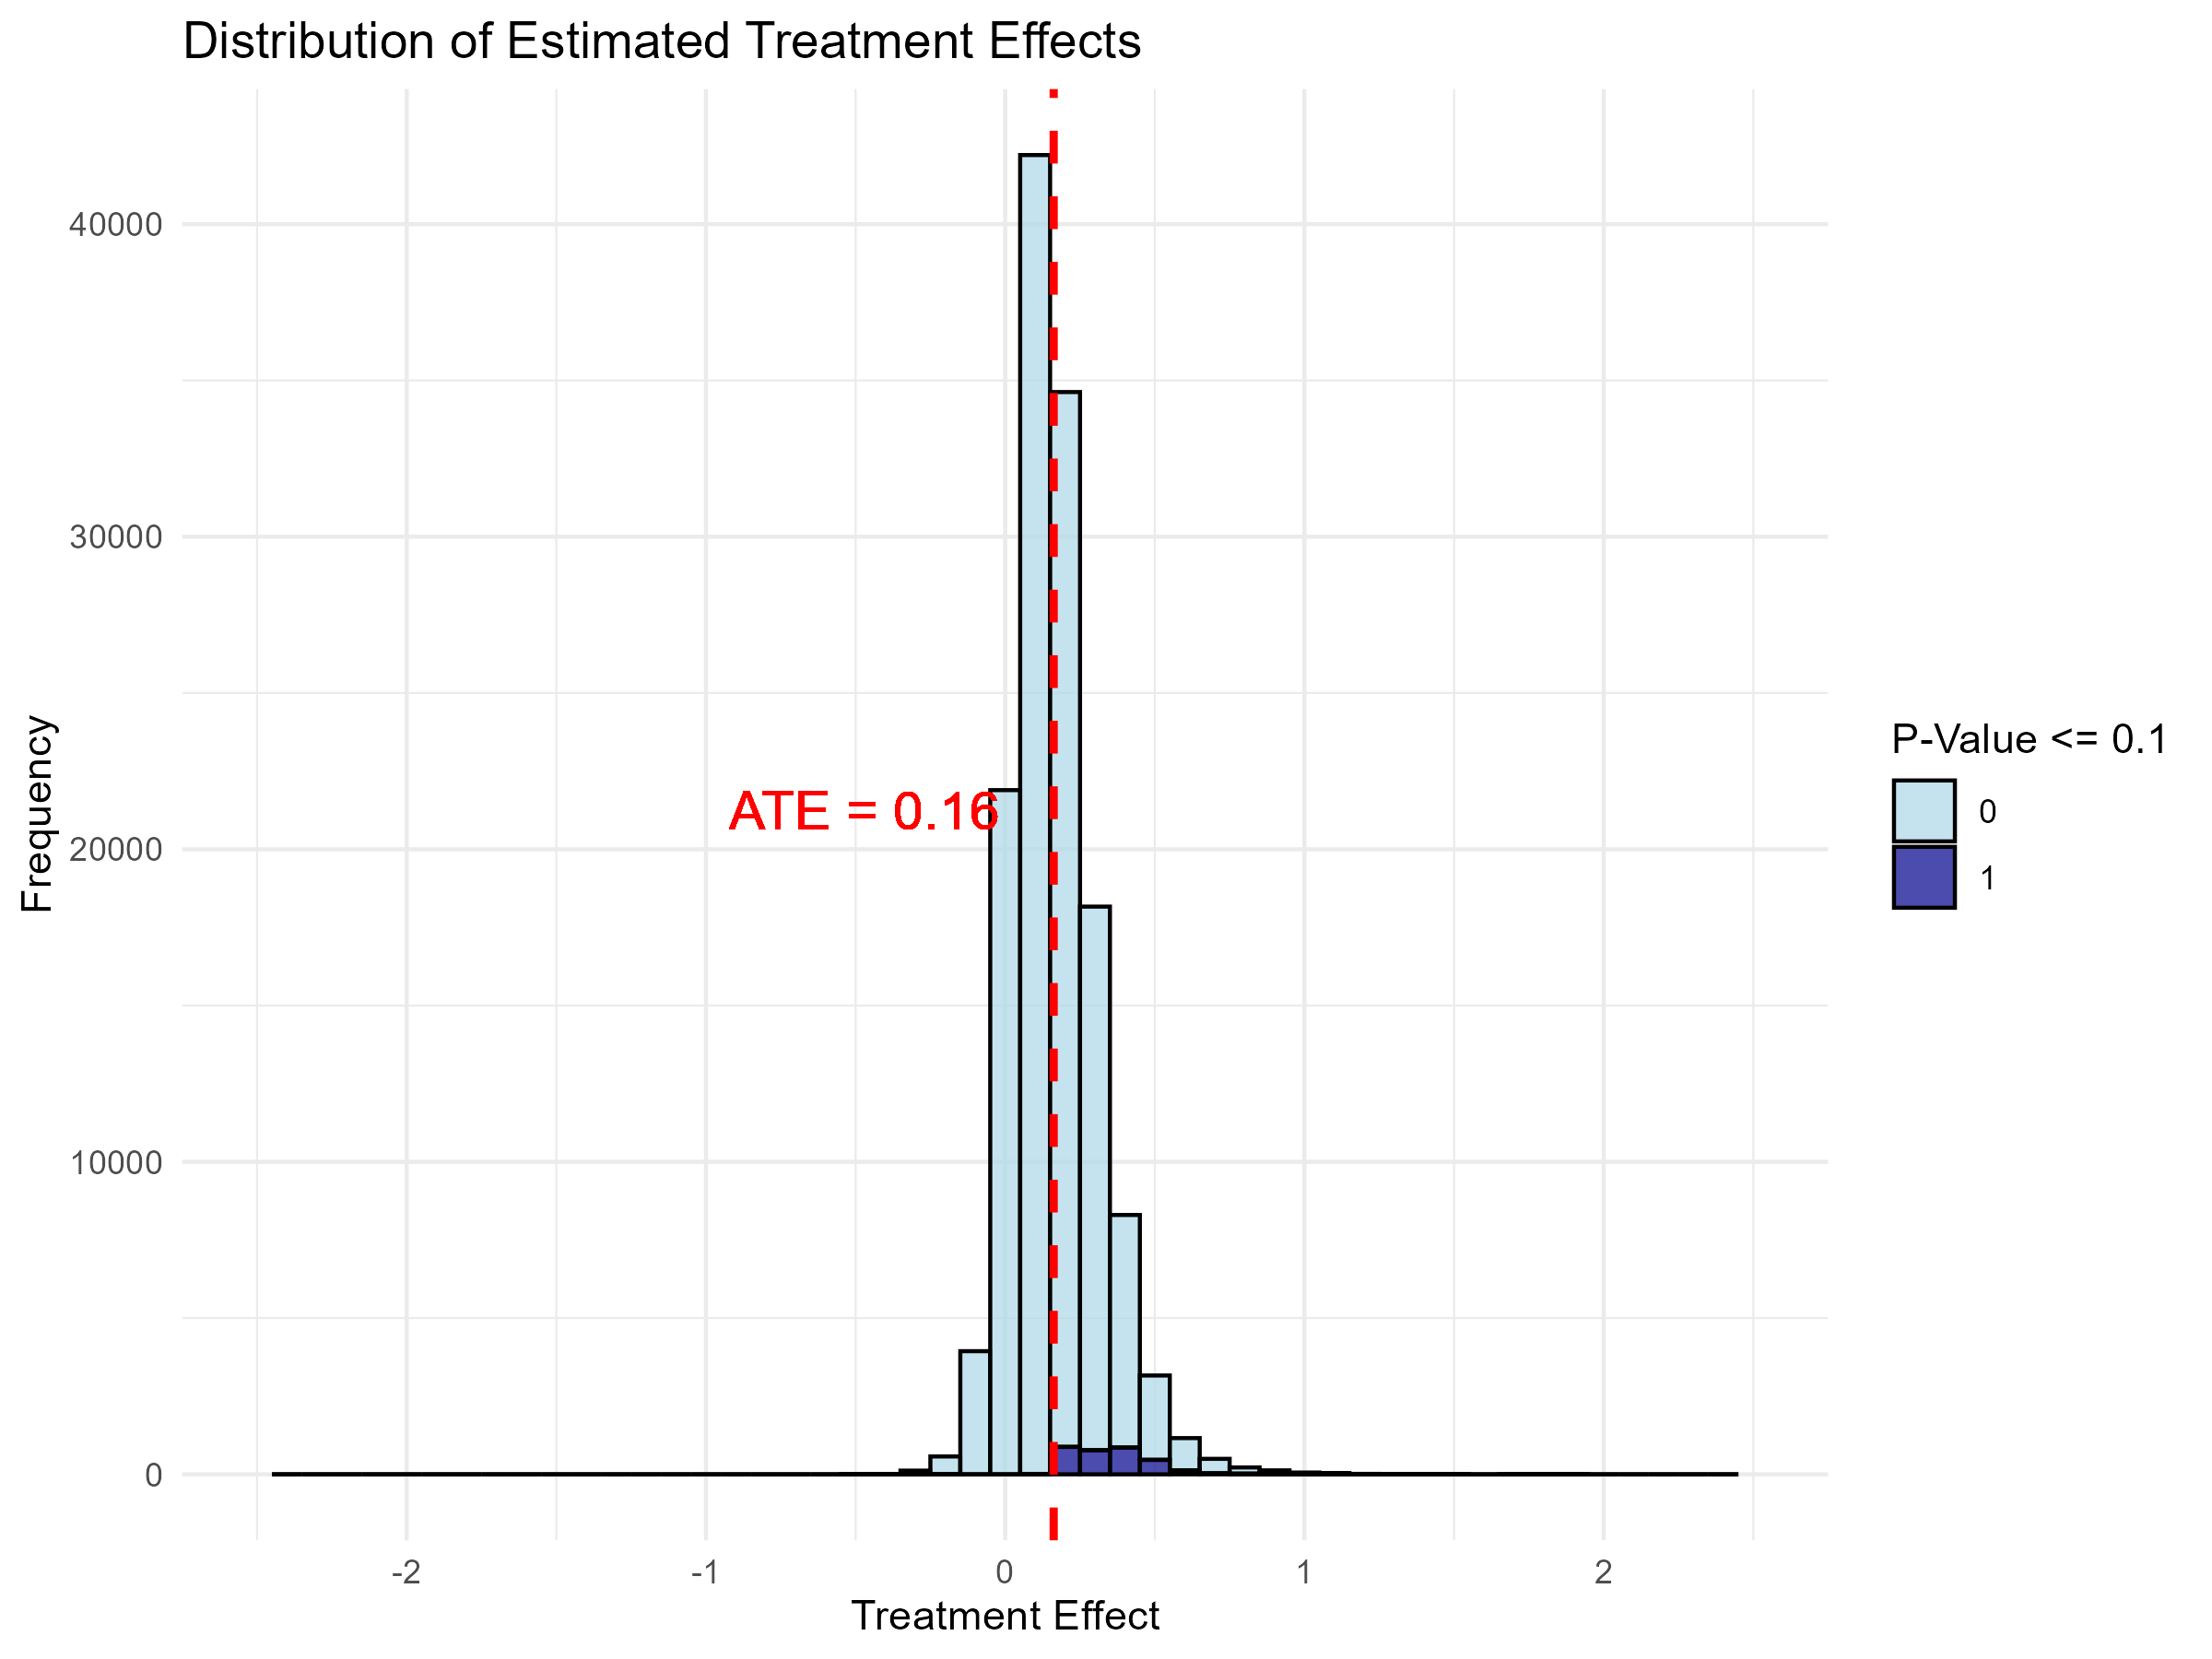
\includegraphics[width=\textwidth]{c:/Users/nickm/OneDrive/Acer (new laptop)/Documents/PhD/Tulane University/Projects/Charter School Heterogeneity/Charter_School_Heterogeneity_Project/analysis/output/figures/cate_dist_afgr.png}
\caption{Treatment Effect Distribution: Graduation Rates}
\label{fig:image2}
\begin{minipage}{1\linewidth}
\singlespacing
\footnotesize
\emph{Notes}: Figure 2 plots the distribution of district $\times$ year treatment effects for graduation rates. These are interrpeted as average partial effects of a given district in a given year. That is, each point represents $\frac{Cov[Y, W | X = x]}{Var[W | X = x]} = E\left[ \frac{\partial \tau(x)}{\partial x} \right]$, the predicted treatment effect from increasing the charter share in year $t$ by 1 percentage point.
\end{minipage}
\end{figure}

	

Table 1: Group covariate means between significantly positive districts vs. significantly negative districts\\
\begin{table}[!h]
\centering
\caption{\label{tab:cov_means_afgr}Comparing Covariate Means: Graduation Rates}
\centering
\begin{tabular}[t]{lccc}
\toprule
Covariate & \makecell[c]{Significantly\\Positive} & \makecell[c]{Significantly\\Negative} & \makecell[c]{Difference\\(Positive - Negative)}\\
\midrule
\cellcolor{gray!10}{Log of Enrollment} & \cellcolor{gray!10}{7.23} & \cellcolor{gray!10}{6.98} & \cellcolor{gray!10}{0.26**}\\
White (\%) & 0.82 & 0.48 & 0.35***\\
\cellcolor{gray!10}{Black (\%)} & \cellcolor{gray!10}{0.05} & \cellcolor{gray!10}{0.39} & \cellcolor{gray!10}{-0.34***}\\
Hispanic (\%) & 0.09 & 0.05 & 0.04***\\
\cellcolor{gray!10}{Free/Reduced Lunch (\%)} & \cellcolor{gray!10}{0.25} & \cellcolor{gray!10}{0.48} & \cellcolor{gray!10}{-0.23***}\\
Special Ed (\%) & 0.26 & 0.13 & 0.13***\\
\cellcolor{gray!10}{Baseline Performance} & \cellcolor{gray!10}{0.83} & \cellcolor{gray!10}{0.57} & \cellcolor{gray!10}{0.26***}\\
Urban & 0.07 & 0.07 & 0\\
\cellcolor{gray!10}{Suburb} & \cellcolor{gray!10}{0.22} & \cellcolor{gray!10}{0.14} & \cellcolor{gray!10}{0.08***}\\
Town & 0.22 & 0.17 & 0.06*\\
\cellcolor{gray!10}{Rural} & \cellcolor{gray!10}{0.48} & \cellcolor{gray!10}{0.62} & \cellcolor{gray!10}{-0.14***}\\
Magnet Schools (\%) & 0.18 & 0.01 & 0.17\\
\cellcolor{gray!10}{City Population (standardized)} & \cellcolor{gray!10}{0.00} & \cellcolor{gray!10}{0.00} & \cellcolor{gray!10}{0}\\
University in City & -0.01 & 0.01 & -0.01**\\
\cellcolor{gray!10}{Per Pupil Revenue} & \cellcolor{gray!10}{11411.08} & \cellcolor{gray!10}{8940.67} & \cellcolor{gray!10}{2470.41***}\\
Student-Teacher Ratio & 14.20 & 14.93 & -0.73***\\
\cellcolor{gray!10}{Teacher Salary} & \cellcolor{gray!10}{81975.53} & \cellcolor{gray!10}{65372.43} & \cellcolor{gray!10}{16603.09***}\\
TPS-Charter Spending (\% diff) & 0.03 & 0.01 & 0.02***\\
\cellcolor{gray!10}{Total Spending (per-pupil)} & \cellcolor{gray!10}{11480.57} & \cellcolor{gray!10}{9178.68} & \cellcolor{gray!10}{2301.89***}\\
Equitable Funding & 6.21 & 5.06 & 1.15***\\
\cellcolor{gray!10}{No Caps on CS Growth} & \cellcolor{gray!10}{8.26} & \cellcolor{gray!10}{9.12} & \cellcolor{gray!10}{-0.86***}\\
Performance-Based Contracts & 8.31 & 9.75 & -1.44***\\
\cellcolor{gray!10}{Transparent Charter Startup Policies} & \cellcolor{gray!10}{7.98} & \cellcolor{gray!10}{10.16} & \cellcolor{gray!10}{-2.18***}\\
Clear Charter Renewal Policies & 10.54 & 11.91 & -1.37***\\
\cellcolor{gray!10}{Exempt from State/District Regs} & \cellcolor{gray!10}{7.51} & \cellcolor{gray!10}{8.04} & \cellcolor{gray!10}{-0.53***}\\
\midrule
Number of Observations & 438.00 & 277.00 & 715\\
\bottomrule
\end{tabular}
\end{table}
\\

Table \ref{tab:state_gates_afgr}: Avg treatment effects within US states\\
\begin{table}[!h]
\centering
\caption{\label{tab:state_gates_afgr}GATEs within States (Graduation Rates)}
\centering
\begin{tabular}[t]{llrrr}
\toprule
State & GATE & SE & p.value & Share.of.N\\
\midrule
\cellcolor{gray!10}{Alabama} & \cellcolor{gray!10}{0.206***} & \cellcolor{gray!10}{0.039} & \cellcolor{gray!10}{0.000} & \cellcolor{gray!10}{0.012}\\
Alaska & -0.618* & 0.342 & 0.070 & 0.004\\
\cellcolor{gray!10}{Arizona} & \cellcolor{gray!10}{-0.198} & \cellcolor{gray!10}{0.155} & \cellcolor{gray!10}{0.199} & \cellcolor{gray!10}{0.012}\\
Arkansas & -1.085** & 0.517 & 0.036 & 0.025\\
\cellcolor{gray!10}{California} & \cellcolor{gray!10}{-0.054} & \cellcolor{gray!10}{0.057} & \cellcolor{gray!10}{0.339} & \cellcolor{gray!10}{0.046}\\
Colorado & 0.034 & 0.077 & 0.662 & 0.019\\
\cellcolor{gray!10}{Connecticut} & \cellcolor{gray!10}{0.185***} & \cellcolor{gray!10}{0.048} & \cellcolor{gray!10}{0.000} & \cellcolor{gray!10}{0.012}\\
Delaware & 0.69*** & 0.214 & 0.001 & 0.002\\
\cellcolor{gray!10}{Florida} & \cellcolor{gray!10}{0.192***} & \cellcolor{gray!10}{0.071} & \cellcolor{gray!10}{0.007} & \cellcolor{gray!10}{0.007}\\
Georgia & -0.093 & 0.165 & 0.572 & 0.018\\
\cellcolor{gray!10}{Idaho} & \cellcolor{gray!10}{-0.148} & \cellcolor{gray!10}{0.198} & \cellcolor{gray!10}{0.454} & \cellcolor{gray!10}{0.012}\\
Illinois & 0.189*** & 0.025 & 0.000 & 0.052\\
\cellcolor{gray!10}{Indiana} & \cellcolor{gray!10}{0.093***} & \cellcolor{gray!10}{0.029} & \cellcolor{gray!10}{0.002} & \cellcolor{gray!10}{0.032}\\
Kansas & -1.537** & 0.629 & 0.014 & 0.031\\
\cellcolor{gray!10}{Kentucky} & \cellcolor{gray!10}{0.197***} & \cellcolor{gray!10}{0.029} & \cellcolor{gray!10}{0.000} & \cellcolor{gray!10}{0.017}\\
Louisiana & 0.033 & 0.107 & 0.756 & 0.007\\
\cellcolor{gray!10}{Maine} & \cellcolor{gray!10}{0.121***} & \cellcolor{gray!10}{0.020} & \cellcolor{gray!10}{0.000} & \cellcolor{gray!10}{0.012}\\
Massachusetts & 0.073 & 0.058 & 0.203 & 0.025\\
\cellcolor{gray!10}{Michigan} & \cellcolor{gray!10}{0.101***} & \cellcolor{gray!10}{0.033} & \cellcolor{gray!10}{0.003} & \cellcolor{gray!10}{0.057}\\
Minnesota & 0.24*** & 0.066 & 0.000 & 0.034\\
\cellcolor{gray!10}{Mississippi} & \cellcolor{gray!10}{0.246***} & \cellcolor{gray!10}{0.030} & \cellcolor{gray!10}{0.000} & \cellcolor{gray!10}{0.013}\\
Montana & 0.14*** & 0.021 & 0.000 & 0.017\\
\cellcolor{gray!10}{Nebraska} & \cellcolor{gray!10}{0.132***} & \cellcolor{gray!10}{0.012} & \cellcolor{gray!10}{0.000} & \cellcolor{gray!10}{0.025}\\
Nevada & -0.174 & 0.193 & 0.369 & 0.002\\
\cellcolor{gray!10}{New Hampshire} & \cellcolor{gray!10}{0.461**} & \cellcolor{gray!10}{0.200} & \cellcolor{gray!10}{0.021} & \cellcolor{gray!10}{0.007}\\
New Jersey & 0.126*** & 0.023 & 0.000 & 0.027\\
\cellcolor{gray!10}{New Mexico} & \cellcolor{gray!10}{-0.434} & \cellcolor{gray!10}{0.317} & \cellcolor{gray!10}{0.172} & \cellcolor{gray!10}{0.010}\\
New York & 0.156*** & 0.019 & 0.000 & 0.070\\
\cellcolor{gray!10}{North Carolina} & \cellcolor{gray!10}{0.137} & \cellcolor{gray!10}{0.087} & \cellcolor{gray!10}{0.115} & \cellcolor{gray!10}{0.012}\\
North Dakota & 0.143*** & 0.024 & 0.000 & 0.015\\
\cellcolor{gray!10}{Ohio} & \cellcolor{gray!10}{0.177***} & \cellcolor{gray!10}{0.029} & \cellcolor{gray!10}{0.000} & \cellcolor{gray!10}{0.067}\\
Oregon & -0.161 & 0.316 & 0.611 & 0.019\\
\cellcolor{gray!10}{Pennsylvania} & \cellcolor{gray!10}{0.147***} & \cellcolor{gray!10}{0.050} & \cellcolor{gray!10}{0.004} & \cellcolor{gray!10}{0.055}\\
South Carolina & 0.01 & 0.121 & 0.933 & 0.009\\
\cellcolor{gray!10}{South Dakota} & \cellcolor{gray!10}{0.156***} & \cellcolor{gray!10}{0.035} & \cellcolor{gray!10}{0.000} & \cellcolor{gray!10}{0.016}\\
Texas & 0.206*** & 0.031 & 0.000 & 0.103\\
\cellcolor{gray!10}{Utah} & \cellcolor{gray!10}{0.075} & \cellcolor{gray!10}{0.114} & \cellcolor{gray!10}{0.507} & \cellcolor{gray!10}{0.004}\\
Vermont & 0.152*** & 0.030 & 0.000 & 0.005\\
\cellcolor{gray!10}{Virginia} & \cellcolor{gray!10}{0.137***} & \cellcolor{gray!10}{0.033} & \cellcolor{gray!10}{0.000} & \cellcolor{gray!10}{0.014}\\
Washington & 0.205*** & 0.039 & 0.000 & 0.027\\
\cellcolor{gray!10}{West Virginia} & \cellcolor{gray!10}{0.143**} & \cellcolor{gray!10}{0.064} & \cellcolor{gray!10}{0.025} & \cellcolor{gray!10}{0.006}\\
Wisconsin & 0.254*** & 0.046 & 0.000 & 0.042\\
\bottomrule
\end{tabular}
\end{table}
\\


Table 3: Avg treatment effects of pre-specified subgroups\\
% latex table generated in R 4.4.0 by xtable 1.8-4 package
% Fri Sep 20 11:07:44 2024
\begin{tabular}{rlrrrr}
  \hline
 & Group & GATE & SE & p.value & Share.of.N \\ 
  \hline
1 & Urban &  &  &  & 0.06 \\ 
  2 & Suburban &  &  &  & 0.23 \\ 
  3 & Rural &  &  &  & 0.52 \\ 
  4 & Percent Free Lunch $>$ 20\% &  &  &  & 0.60 \\ 
  5 & Urban &  &  &  & 0.06 \\ 
  6 & Suburban &  &  &  & 0.23 \\ 
  7 & Rural &  &  &  & 0.52 \\ 
  8 & Percent Free Lunch $>$ 20\% &  &  &  & 0.60 \\ 
  9 & Urban &  & 0.05 &  & 0.06 \\ 
  10 & Suburban &  & 0.03 &  & 0.23 \\ 
  11 & Rural &  & 0.09 &  & 0.52 \\ 
  12 & Percent Free Lunch $>$ 20\% &  & 0.04 &  & 0.60 \\ 
   \hline
\end{tabular}
\\

Table 4: Best linear projection $\tau(X) = \alpha + \beta X + e$\\
\begin{table}[!h]
\centering
\caption{\label{tab:blp_afgr}Best Linear Projection: Graduation Rates}
\centering
\begin{tabular}[t]{lcccc}
\toprule
Term & Estimate & Std. Error & t-stat & p-value\\
\midrule
\cellcolor{gray!10}{(Intercept)} & \cellcolor{gray!10}{-2.085**} & \cellcolor{gray!10}{0.901} & \cellcolor{gray!10}{-2.314} & \cellcolor{gray!10}{0.021}\\
Baseline Performance & 0.905** & 0.407 & 2.222 & 0.026\\
\cellcolor{gray!10}{White (\%)} & \cellcolor{gray!10}{-0.002} & \cellcolor{gray!10}{0.300} & \cellcolor{gray!10}{-0.007} & \cellcolor{gray!10}{0.995}\\
Free/Reduced Lunch (\%) & 0.207 & 0.269 & 0.769 & 0.442\\
\cellcolor{gray!10}{TPS-Charter Spending (\% diff)} & \cellcolor{gray!10}{-0.065} & \cellcolor{gray!10}{0.294} & \cellcolor{gray!10}{-0.220} & \cellcolor{gray!10}{0.826}\\
Black (\%) & -0.367 & 0.549 & -0.668 & 0.504\\
\cellcolor{gray!10}{Special Ed (\%)} & \cellcolor{gray!10}{2.992**} & \cellcolor{gray!10}{1.445} & \cellcolor{gray!10}{2.070} & \cellcolor{gray!10}{0.038}\\
Charter Spending (per-pupil) & 0 & 0.000 & -0.466 & 0.641\\
\cellcolor{gray!10}{Log of Enrollment} & \cellcolor{gray!10}{0.132**} & \cellcolor{gray!10}{0.066} & \cellcolor{gray!10}{1.979} & \cellcolor{gray!10}{0.048}\\
Exempt from State/District Regs & -0.019 & 0.031 & -0.590 & 0.555\\
\cellcolor{gray!10}{Hispanic (\%)} & \cellcolor{gray!10}{0.352} & \cellcolor{gray!10}{0.369} & \cellcolor{gray!10}{0.956} & \cellcolor{gray!10}{0.339}\\
\bottomrule
\end{tabular}
\end{table}
\\

\begin{figure}[!h]
\centering
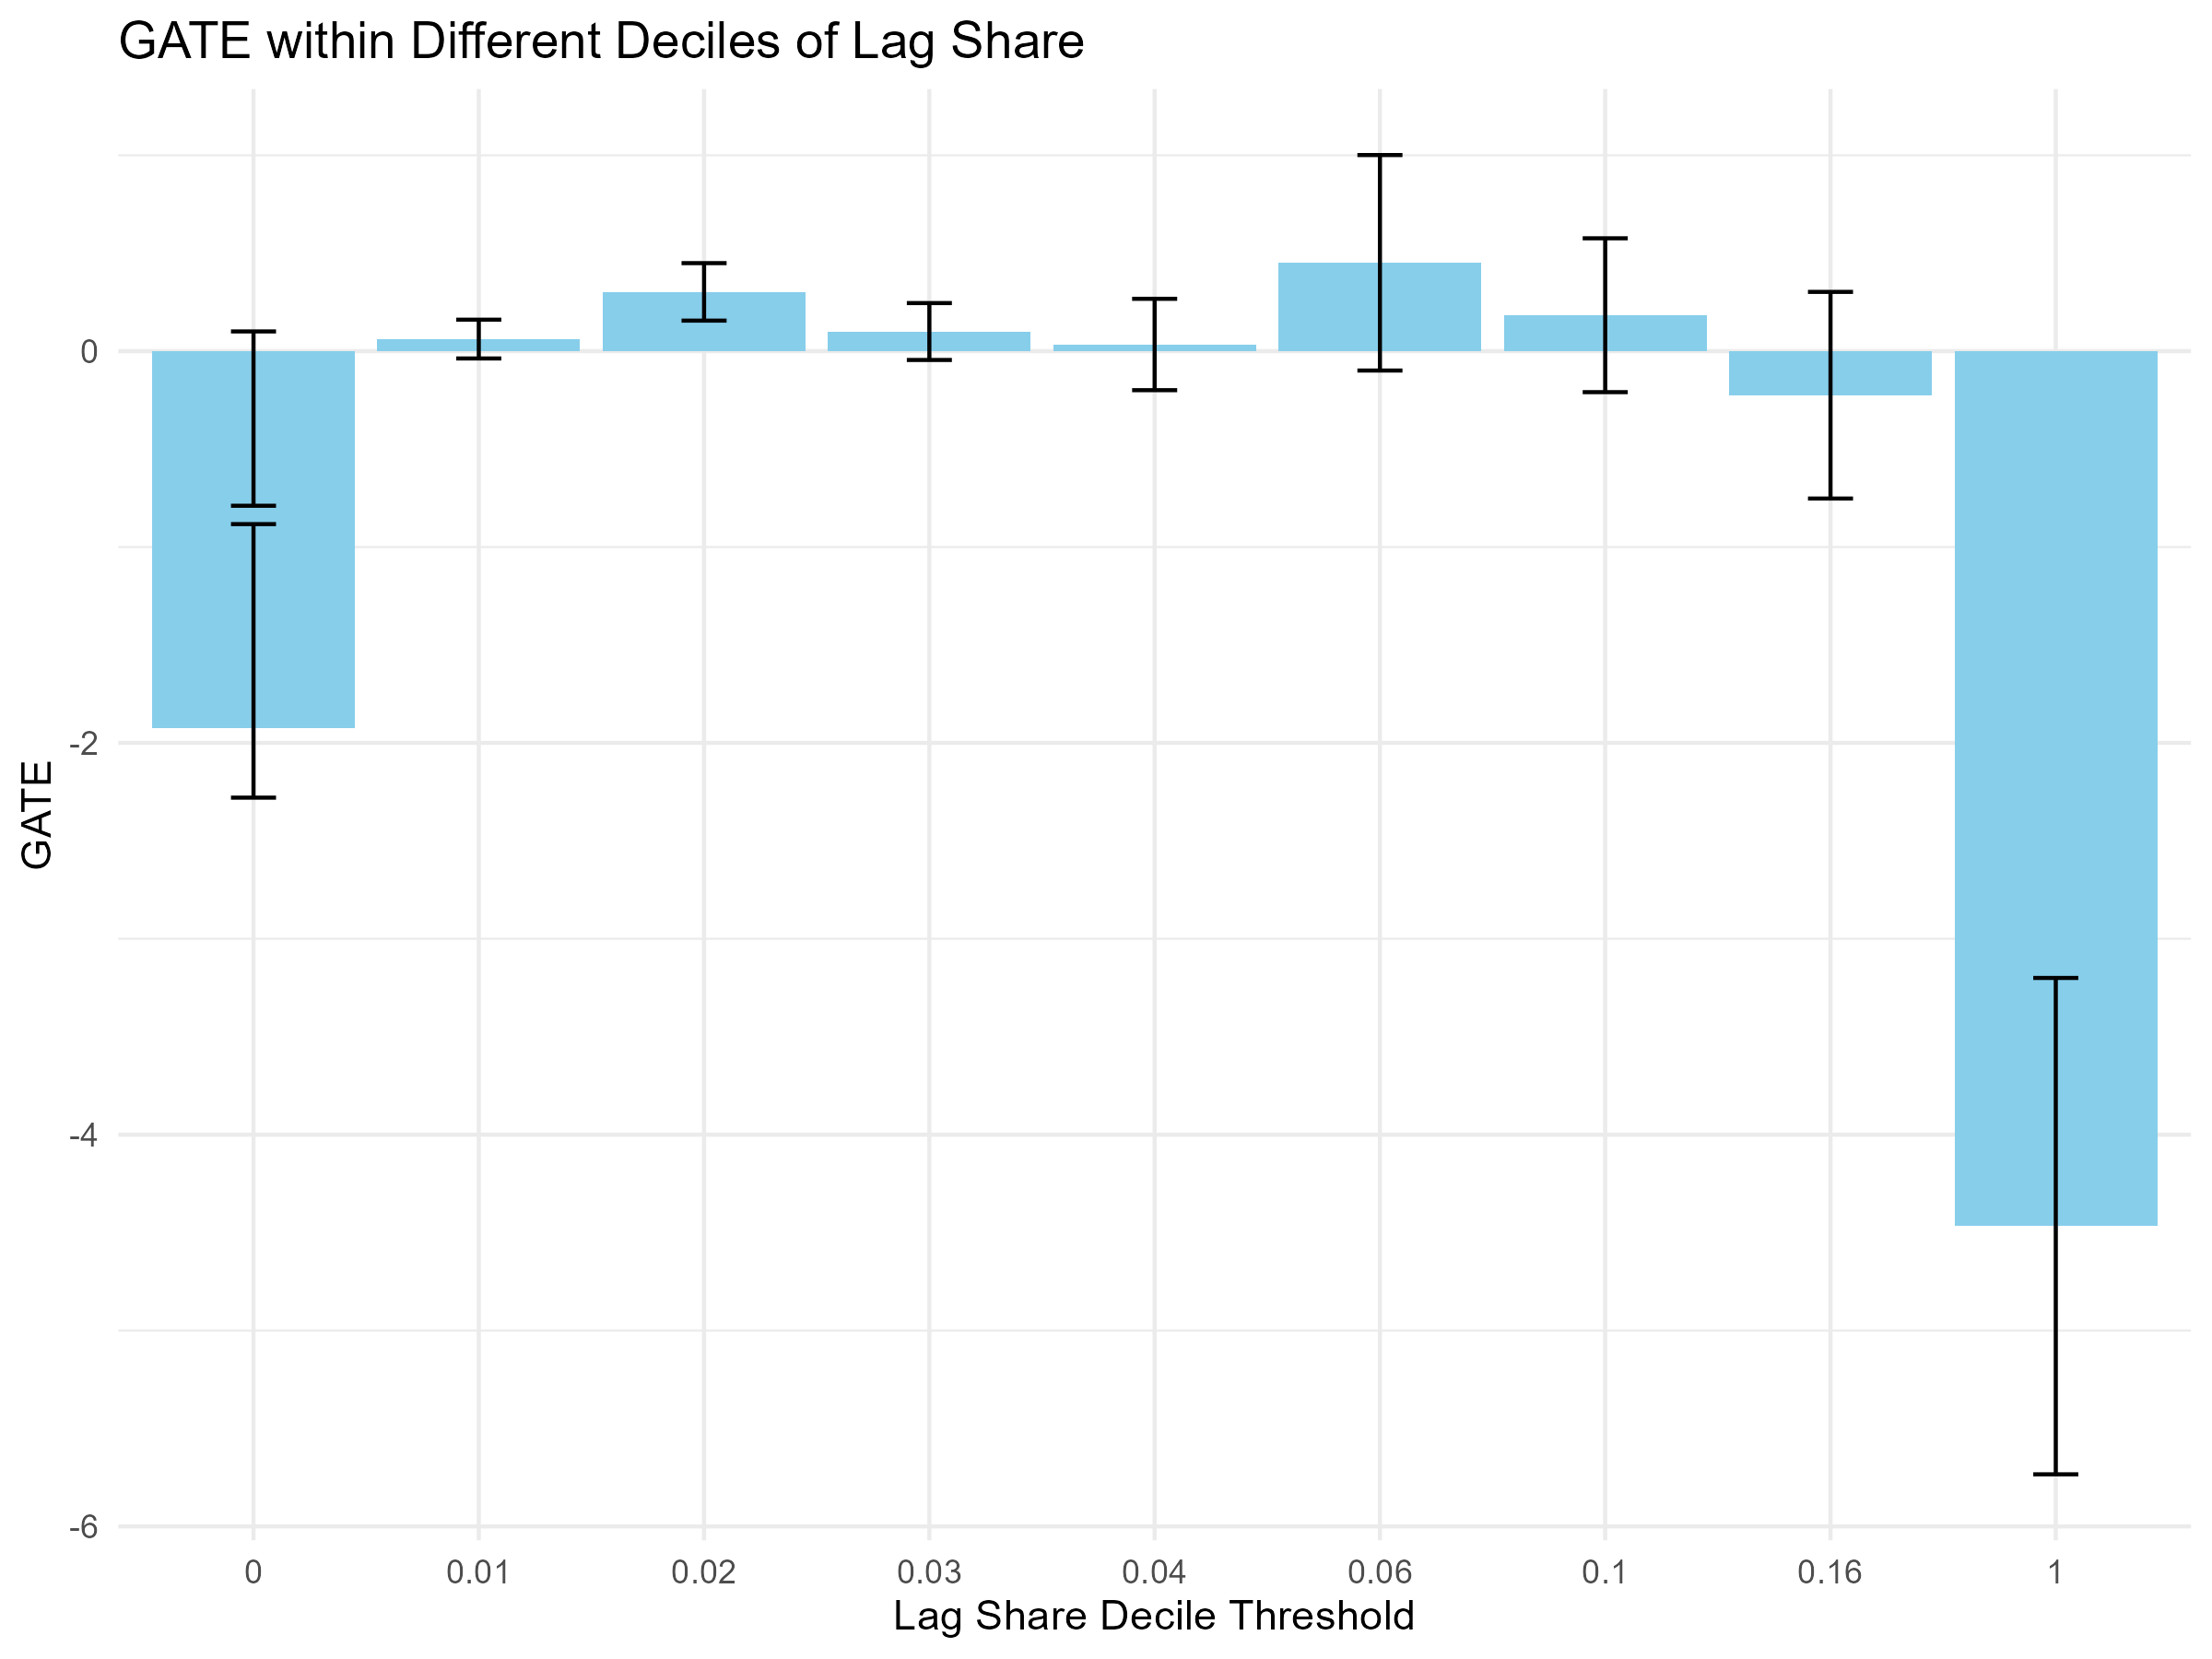
\includegraphics[width=\textwidth]{c:/Users/nickm/OneDrive/Acer (new laptop)/Documents/PhD/Tulane University/Projects/Charter School Heterogeneity/Charter_School_Heterogeneity_Project/analysis/output/figures/gate_deciles_afgr.png}
\caption{Treatment Effects over Dosage Deciles}
\label{fig:dosage_afgr}
\begin{minipage}{1\linewidth}
\singlespacing
\footnotesize
\emph{Notes}: Figure \ref{fig:dosage_afgr} plots the GATE for different deciles of the treatment distribution among treated districts.
\end{minipage}
\end{figure}




	\section{Math Test Scores}

\begin{figure}[H]
\centering
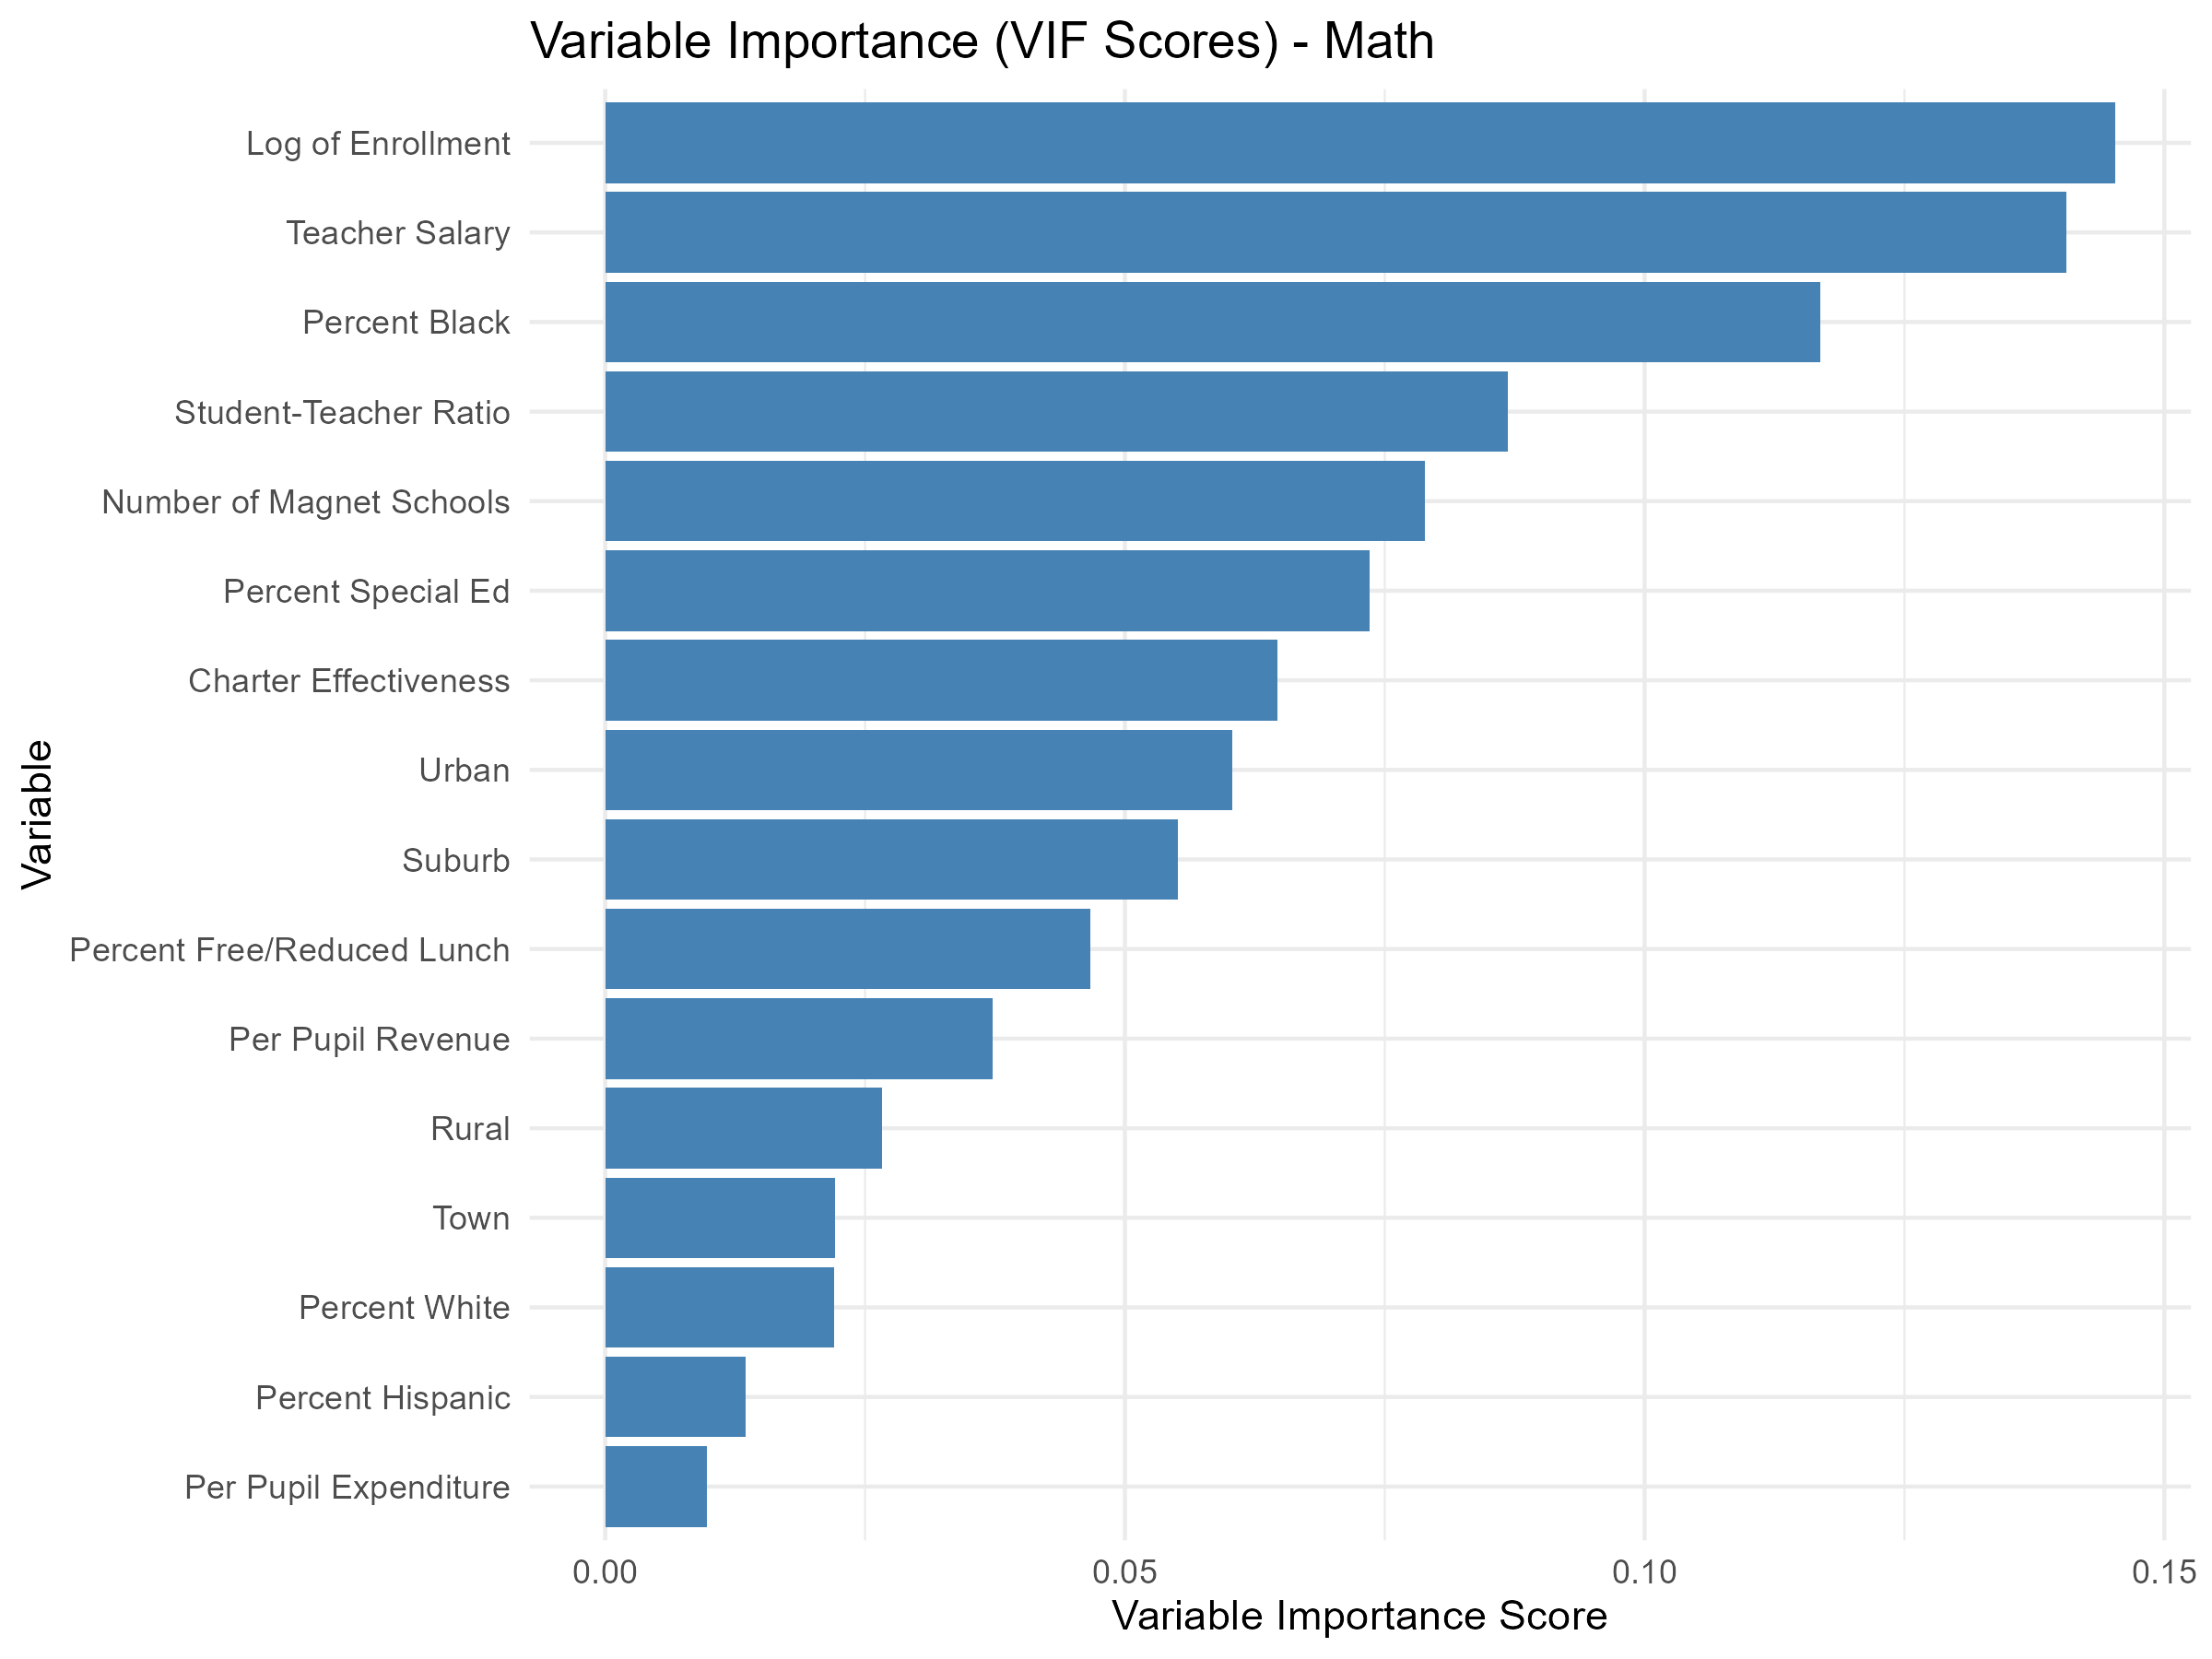
\includegraphics[width=\textwidth]{c:/Users/nickm/OneDrive/Acer (new laptop)/Documents/PhD/Tulane University/Projects/Charter School Heterogeneity/Charter_School_Heterogeneity_Project/analysis/output/figures/vif_scores_math.png}
\caption{VIF Scores: Math Scores}
\label{fig:image3}
\begin{minipage}{1\linewidth}
\singlespacing
\footnotesize
\emph{Notes}: Figure 3 plots VIF scores for Math -- the share of total trees which use a given baseline covariate to perform splitting, weighted by the depth at which the split occurred so that earlier splits within a tree count for slightly more.  
\end{minipage}
\end{figure}


\begin{figure}[H]
\centering
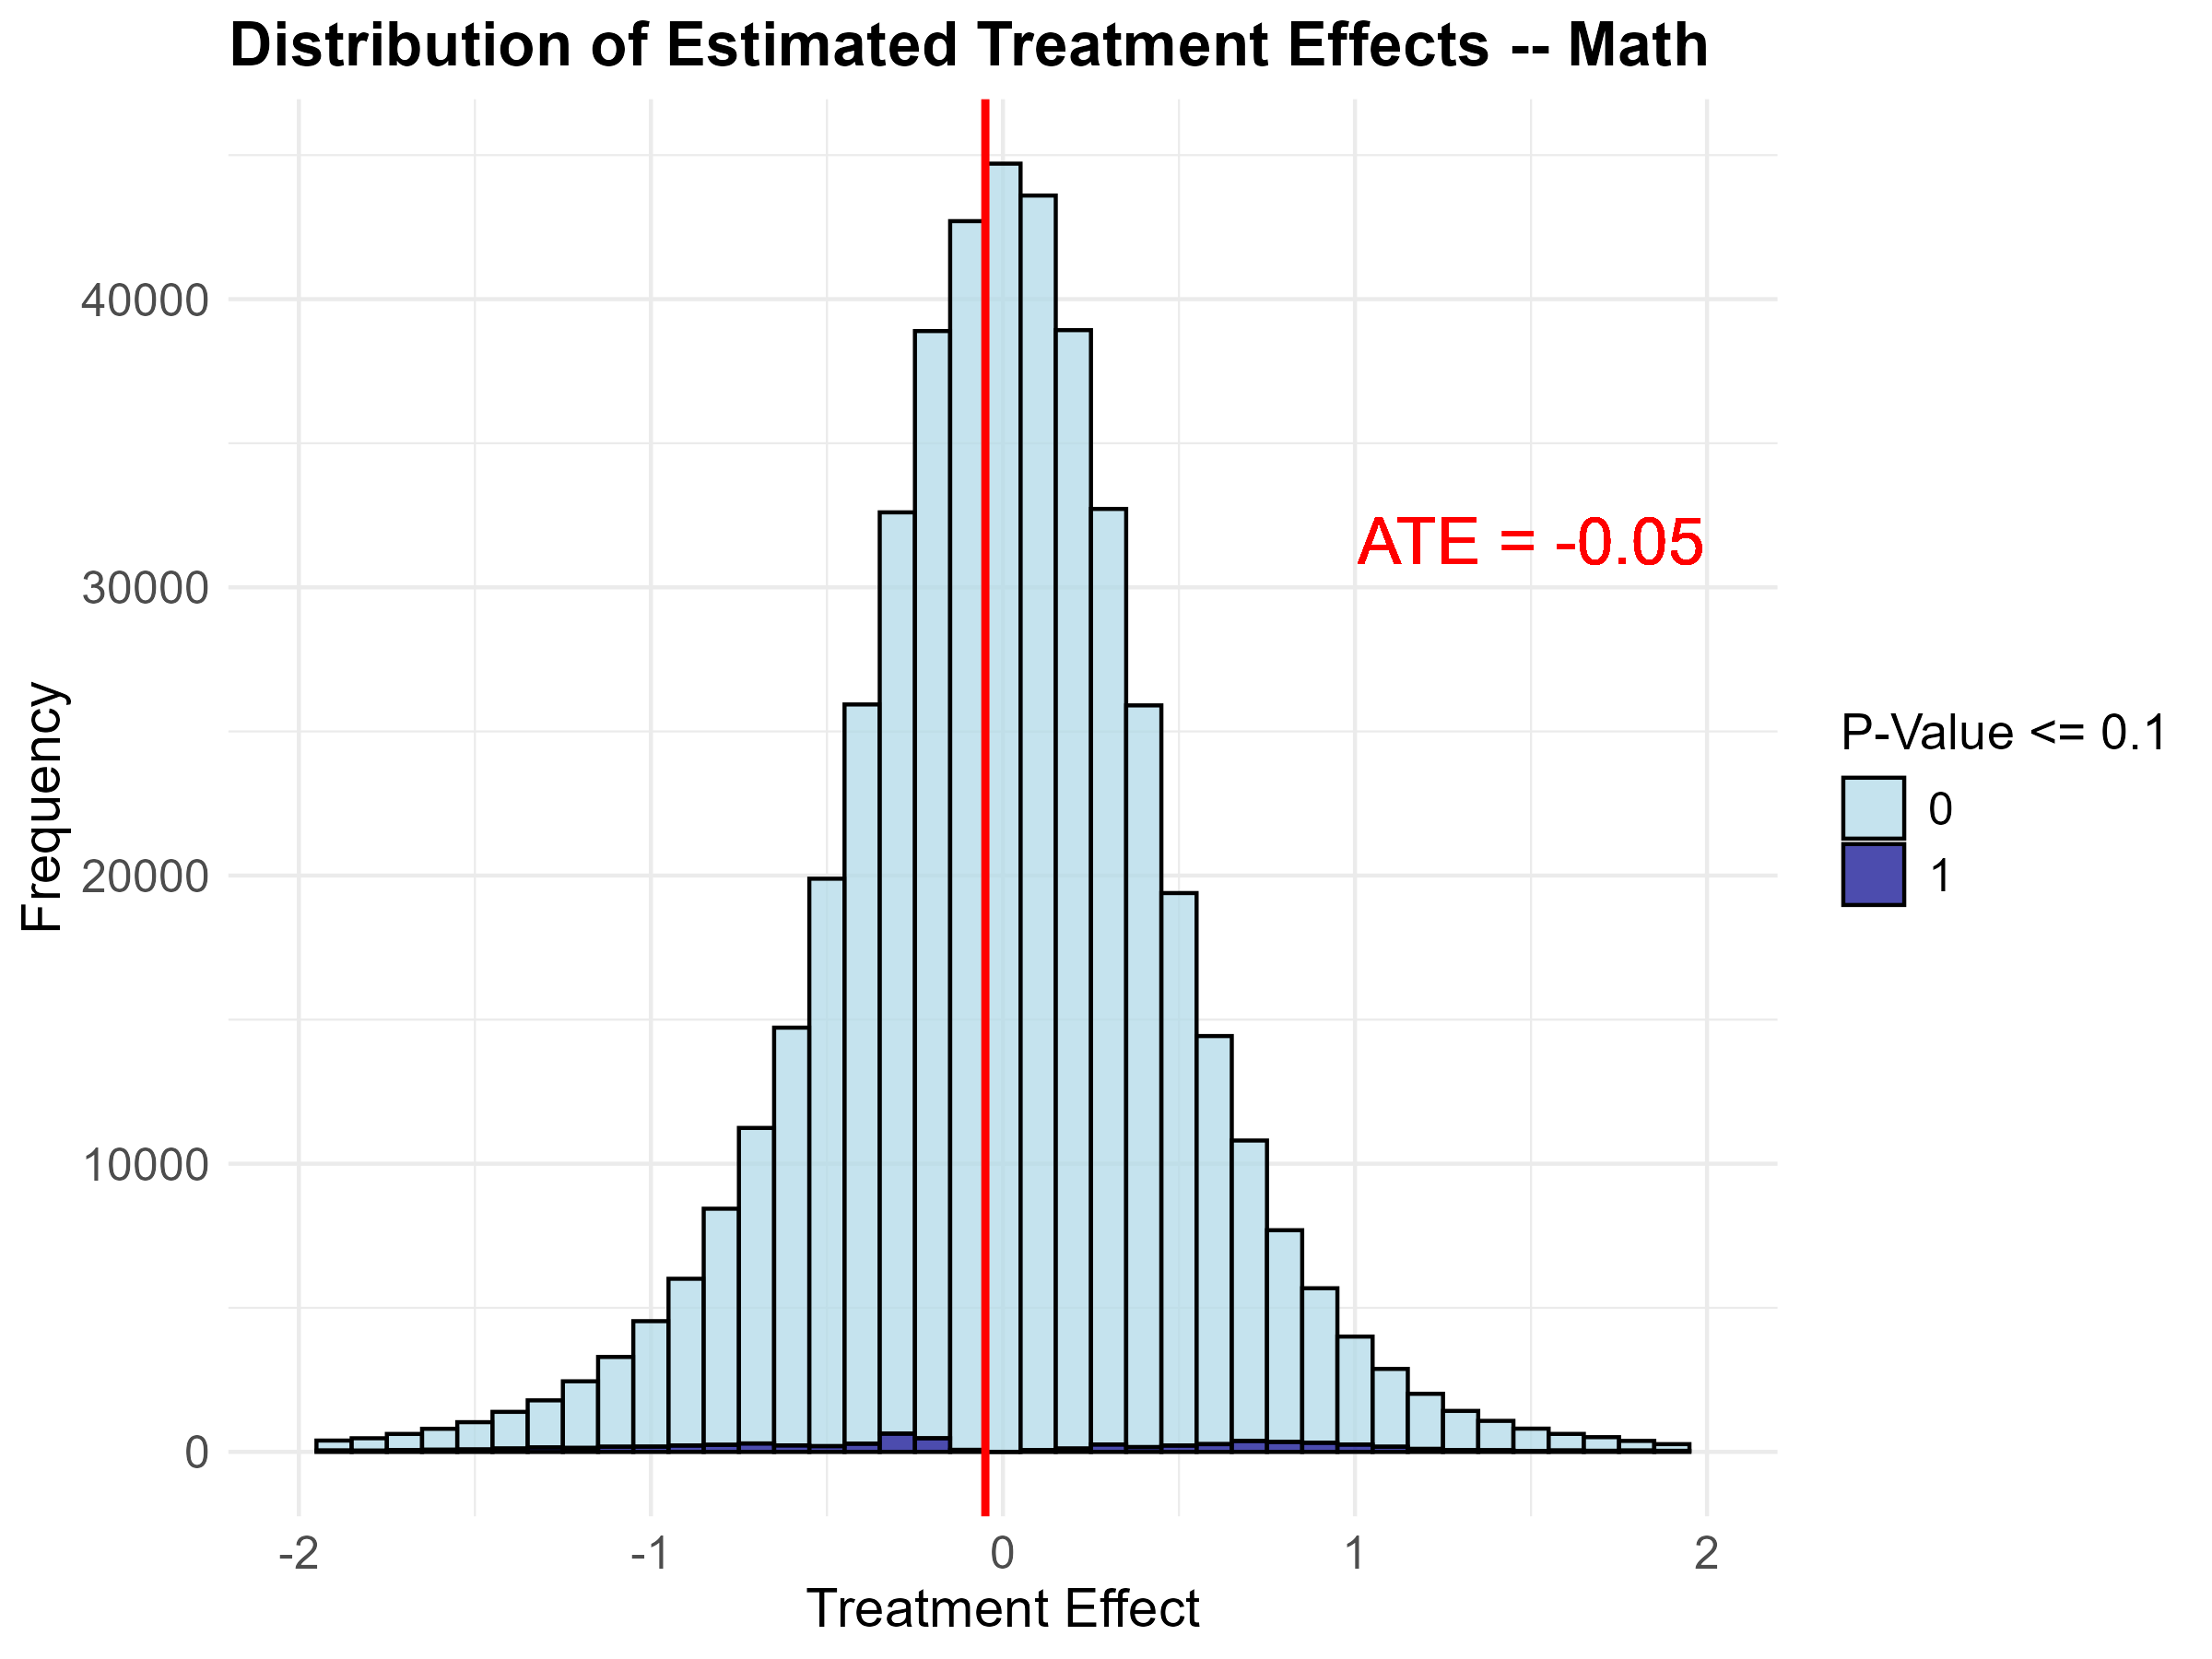
\includegraphics[width=\textwidth]{c:/Users/nickm/OneDrive/Acer (new laptop)/Documents/PhD/Tulane University/Projects/Charter School Heterogeneity/Charter_School_Heterogeneity_Project/analysis/output/figures/cate_dist_math.png}
\caption{Treatment Effect Distribution: Math Scores}
\label{fig:image4}
\begin{minipage}{1\linewidth}
\singlespacing
\footnotesize
\emph{Notes}: Figure 4 plots the distribution of district $\times$ year treatment effects for math scores. These are interrpeted as average partial effects of a given district in a given year. That is, each point represents $\frac{Cov[Y, W | X = x]}{Var[W | X = x]} = E\left[ \frac{\partial \tau(x)}{\partial x} \right]$, the predicted treatment effect from increasing the charter share in year $t$ by 1 percentage point.
\end{minipage}
\end{figure}


Table 4: Group covariate means between significantly positive districts vs. significantly negative districts\\
\begin{table}[!h]
\centering
\caption{\label{tab:cov_means_math}Comparing Covariate Means: Math}
\centering
\begin{tabular}[t]{lccc}
\toprule
Covariate & \makecell[c]{Significantly\\Positive} & \makecell[c]{Significantly\\Negative} & \makecell[c]{Difference\\(Positive - Negative)}\\
\midrule
\cellcolor{gray!10}{Log of Enrollment} & \cellcolor{gray!10}{8.01} & \cellcolor{gray!10}{8.03} & \cellcolor{gray!10}{-0.02***}\\
Percent White & 0.52 & 0.63 & -0.12***\\
\cellcolor{gray!10}{Percent Black} & \cellcolor{gray!10}{0.06} & \cellcolor{gray!10}{0.13} & \cellcolor{gray!10}{-0.07***}\\
Percent Hispanic & 0.31 & 0.19 & 0.12***\\
\cellcolor{gray!10}{Percent Free/Reduced Lunch} & \cellcolor{gray!10}{0.55} & \cellcolor{gray!10}{0.54} & \cellcolor{gray!10}{0.01***}\\
Percent Special Ed & 0.13 & 0.13 & 0***\\
\cellcolor{gray!10}{Urban} & \cellcolor{gray!10}{0.16} & \cellcolor{gray!10}{0.09} & \cellcolor{gray!10}{0.08***}\\
Suburb & 0.28 & 0.32 & -0.04*\\
\cellcolor{gray!10}{Town} & \cellcolor{gray!10}{0.24} & \cellcolor{gray!10}{0.18} & \cellcolor{gray!10}{0.06}\\
Rural & 0.32 & 0.42 & -0.1\\
\cellcolor{gray!10}{Per Pupil Revenue} & \cellcolor{gray!10}{12457.53} & \cellcolor{gray!10}{12154.63} & \cellcolor{gray!10}{302.9*}\\
Per Pupil Expenditure & 12214.59 & 12365.01 & -150.42**\\
\cellcolor{gray!10}{Student-Teacher Ratio} & \cellcolor{gray!10}{18.24} & \cellcolor{gray!10}{17.11} & \cellcolor{gray!10}{1.13***}\\
Teacher Salary & 102784.10 & 97545.43 & 5238.66***\\
\cellcolor{gray!10}{Number of Magnet Schools} & \cellcolor{gray!10}{0.04} & \cellcolor{gray!10}{0.77} & \cellcolor{gray!10}{-0.73}\\
Charter Effectiveness & 0.97 & 0.95 & 0.02\\
\cellcolor{gray!10}{Baseline Performance} & \cellcolor{gray!10}{-0.24} & \cellcolor{gray!10}{-0.20} & \cellcolor{gray!10}{-0.04***}\\
\midrule
Number of Observations & 692.00 & 370.00 & 1062\\
\bottomrule
\end{tabular}
\end{table}
\\


Table 5: Avg treatment effects of pre-specified subgroups \\
% latex table generated in R 4.4.0 by xtable 1.8-4 package
% Thu Oct 31 22:58:37 2024
\begin{tabular}{rlrrrr}
  \hline
 & Group & GATE & SE & p.value & Share.of.N \\ 
  \hline
1 & Urban & 0.02 & 0.11 & 0.89 & 0.06 \\ 
  2 & Suburban & 0.02 & 0.05 & 0.66 & 0.27 \\ 
  3 & Rural & -0.07 & 0.05 & 0.14 & 0.48 \\ 
  4 & Percent Free Lunch $>$ 20\% & -0.04 & 0.03 & 0.23 & 0.87 \\ 
   \hline
\end{tabular}
\\

Table 6: Best linear projection $\tau(X) = \alpha + \beta X + e$\\
\begin{table}[!h]
\centering
\caption{\label{tab:blp_math}Best Linear Projection: Math Scores}
\centering
\begin{tabular}[t]{lcccc}
\toprule
Term & Estimate & Std. Error & t-stat & p-value\\
\midrule
\cellcolor{gray!10}{(Intercept)} & \cellcolor{gray!10}{1.389} & \cellcolor{gray!10}{0.911} & \cellcolor{gray!10}{1.525} & \cellcolor{gray!10}{0.127}\\
White (\%) & -0.186 & 0.485 & -0.384 & 0.701\\
\cellcolor{gray!10}{Black (\%)} & \cellcolor{gray!10}{0.097} & \cellcolor{gray!10}{0.568} & \cellcolor{gray!10}{0.170} & \cellcolor{gray!10}{0.865}\\
Log of Enrollment & -0.115* & 0.065 & -1.775 & 0.076\\
\cellcolor{gray!10}{Magnet Schools (\%)} & \cellcolor{gray!10}{0.007} & \cellcolor{gray!10}{0.005} & \cellcolor{gray!10}{1.433} & \cellcolor{gray!10}{0.152}\\
Hispanic (\%) & 0.082 & 0.450 & 0.182 & 0.856\\
\cellcolor{gray!10}{TPS-Charter Spending (\% diff)} & \cellcolor{gray!10}{0.211} & \cellcolor{gray!10}{0.193} & \cellcolor{gray!10}{1.093} & \cellcolor{gray!10}{0.274}\\
Baseline Performance & 0.079 & 0.084 & 0.939 & 0.348\\
\cellcolor{gray!10}{Free/Reduced Lunch (\%)} & \cellcolor{gray!10}{0.024} & \cellcolor{gray!10}{0.428} & \cellcolor{gray!10}{0.056} & \cellcolor{gray!10}{0.955}\\
City Population (standardized) & 0.177* & 0.096 & 1.843 & 0.065\\
\cellcolor{gray!10}{Per Pupil Revenue} & \cellcolor{gray!10}{0} & \cellcolor{gray!10}{0.000} & \cellcolor{gray!10}{-1.396} & \cellcolor{gray!10}{0.163}\\
\bottomrule
\end{tabular}
\end{table}
\\


	\section{ELA Test Scores}

\begin{figure}[H]
\centering
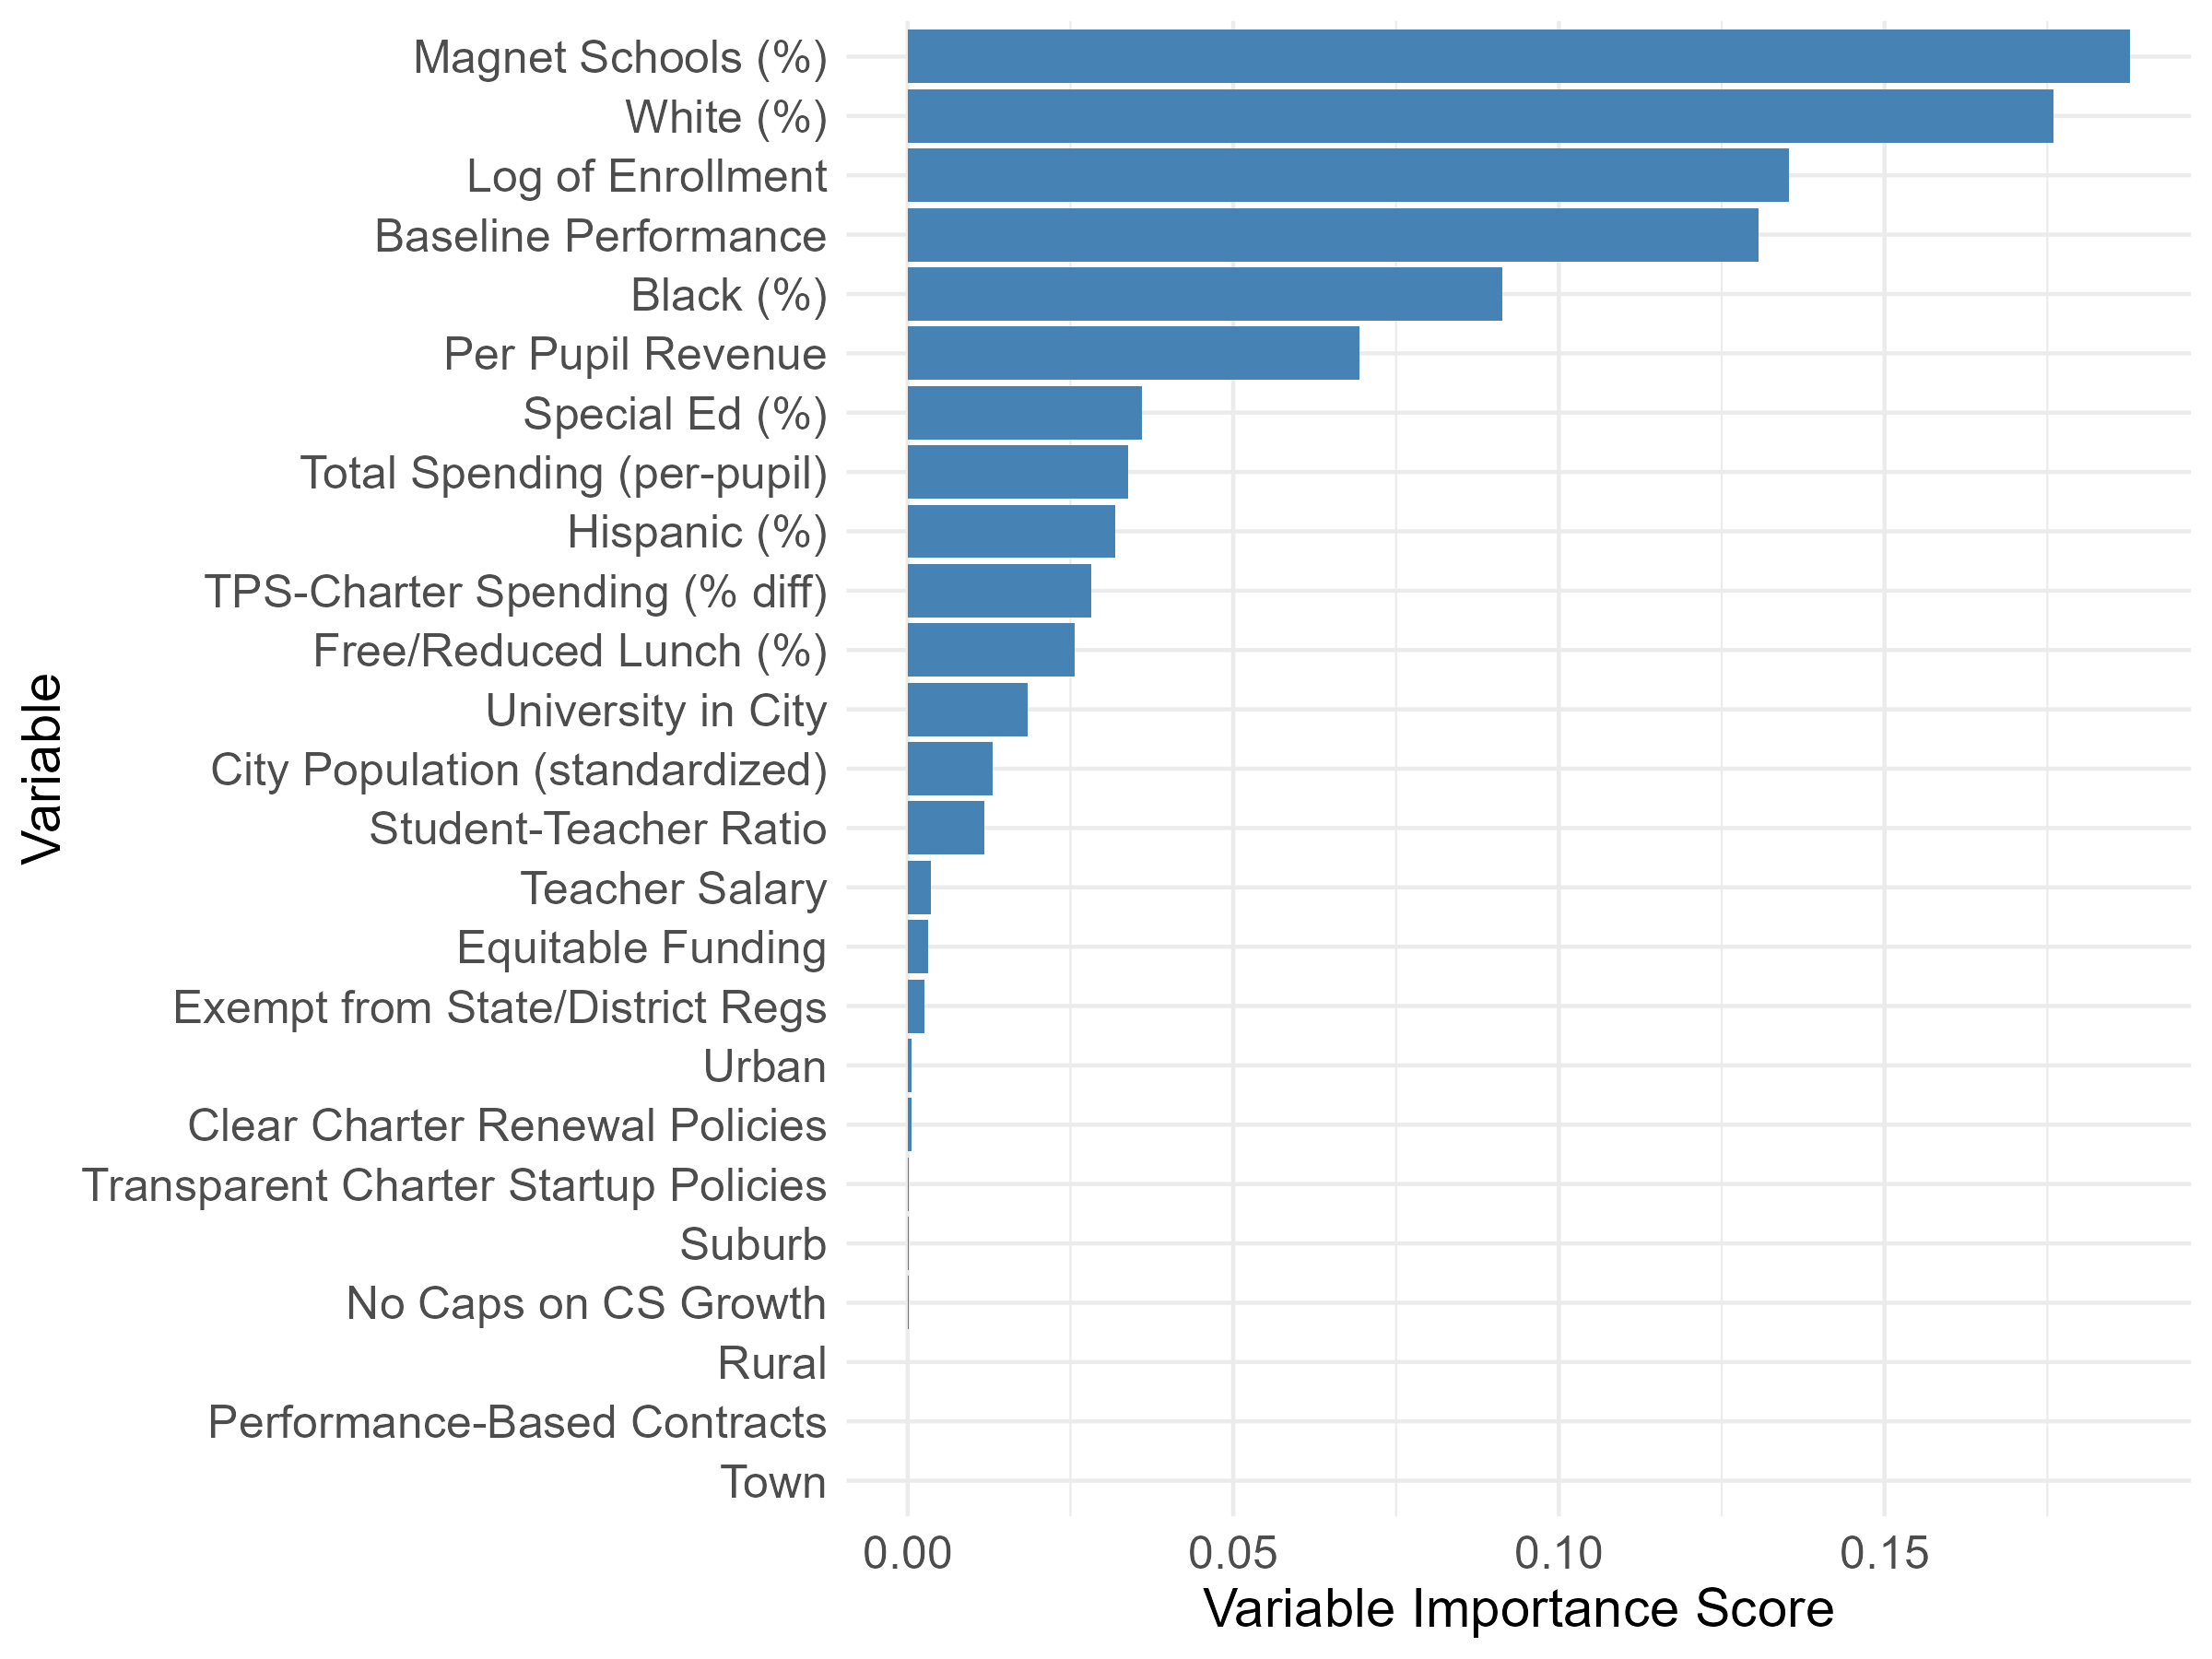
\includegraphics[width=\textwidth]{c:/Users/nickm/OneDrive/Acer (new laptop)/Documents/PhD/Tulane University/Projects/Charter School Heterogeneity/Charter_School_Heterogeneity_Project/analysis/output/figures/vif_scores_ela.png}
\caption{VIF Scores: ELA Scores}
\label{fig:image5}
\begin{minipage}{1\linewidth}
\singlespacing
\footnotesize
\emph{Notes}: Figure 5 plots VIF scores for ELA -- the share of total trees which use a given baseline covariate to perform splitting, weighted by the depth at which the split occurred so that earlier splits within a tree count for slightly more.  
\end{minipage}
\end{figure}


\begin{figure}[H]
\centering
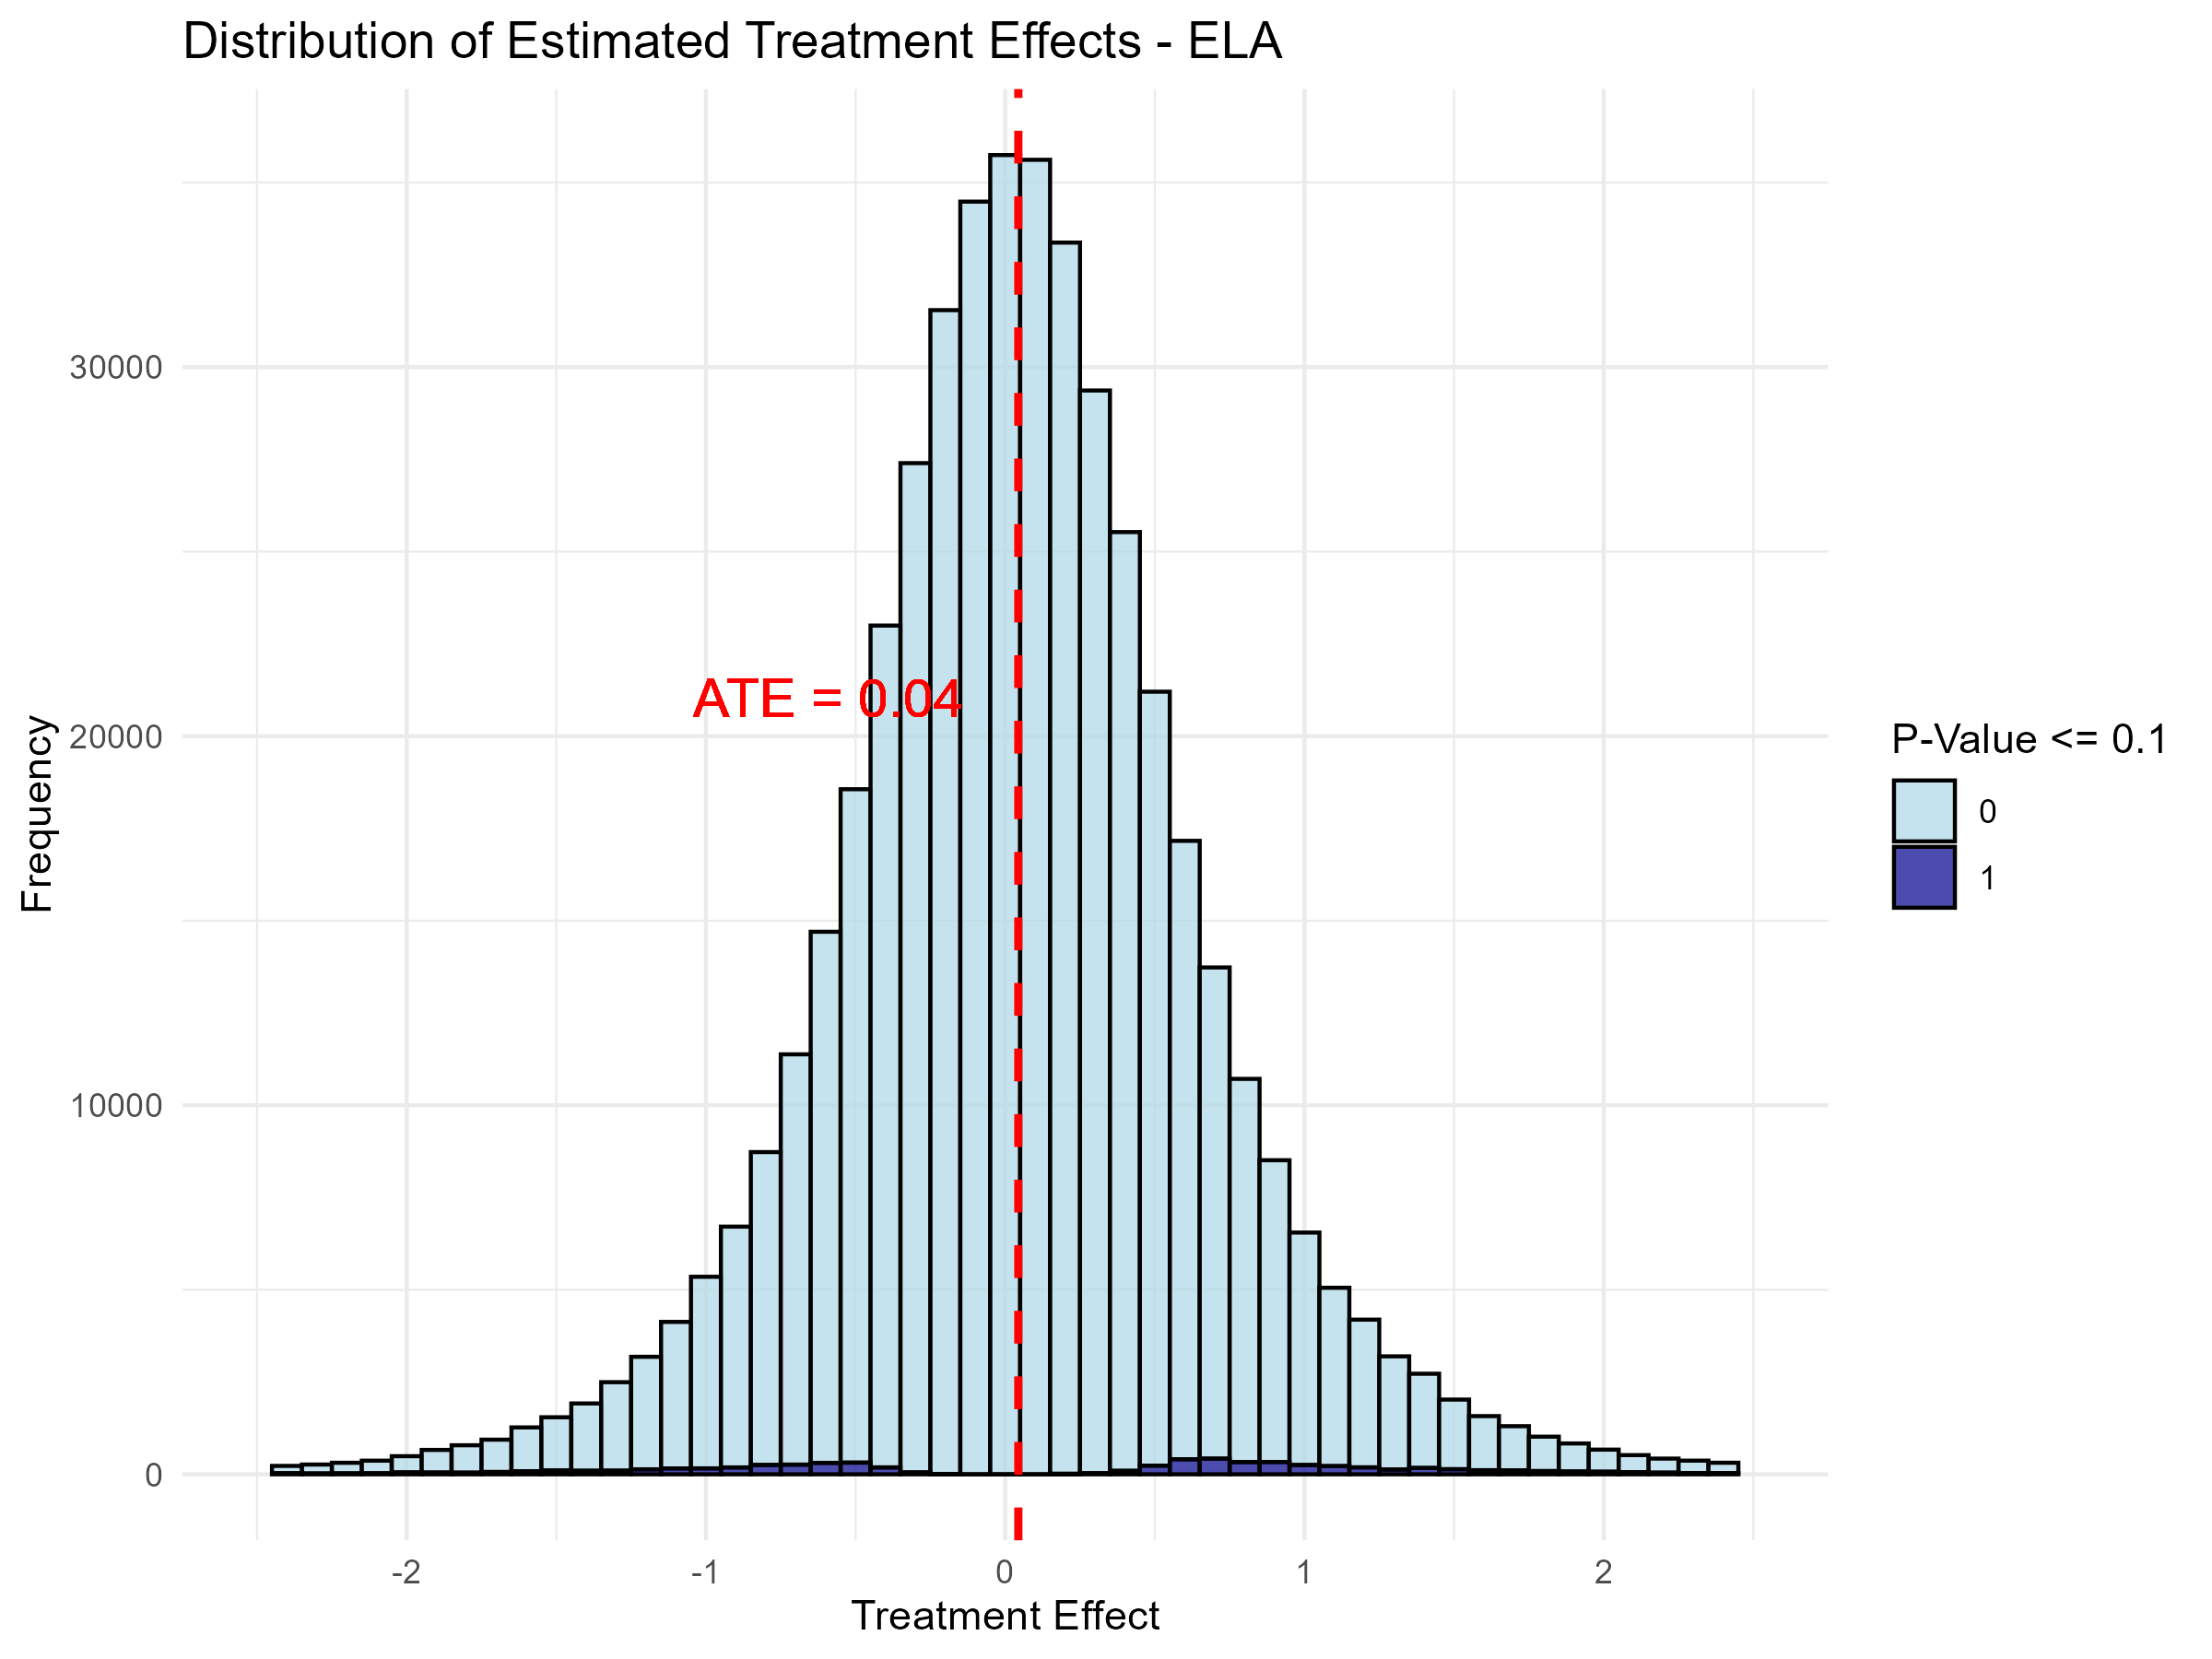
\includegraphics[width=\textwidth]{c:/Users/nickm/OneDrive/Acer (new laptop)/Documents/PhD/Tulane University/Projects/Charter School Heterogeneity/Charter_School_Heterogeneity_Project/analysis/output/figures/cate_dist_ela.png}
\caption{Treatment Effect Distribution: ELA Scores}
\label{fig:image6}
\begin{minipage}{1\linewidth}
\singlespacing
\footnotesize
\emph{Notes}: Figure 6 plots the distribution of district $\times$ year treatment effects for ELA scores. These are interrpeted as average partial effects of a given district in a given year. That is, each point represents $\frac{Cov[Y, W | X = x]}{Var[W | X = x]} = E\left[ \frac{\partial \tau(x)}{\partial x} \right]$, the predicted treatment effect from increasing the charter share in year $t$ by 1 percentage point.
\end{minipage}
\end{figure}



Table 7: Group covariate means between significantly positive districts vs. significantly negative districts\\
% latex table generated in R 4.4.0 by xtable 1.8-4 package
% Fri Sep 20 19:13:30 2024
\begin{tabular}{rlrrr}
  \hline
 & Covariate & Significantly Positive & Significantly Negative & Difference (Positive - Negative) \\ 
  \hline
1 & Log of Enrollment & 8.21 & 7.73 & 0.48 \\ 
  2 & Percent White & 0.42 & 0.68 & -0.25 \\ 
  3 & Percent Black & 0.07 & 0.12 & -0.04 \\ 
  4 & Percent Hispanic & 0.39 & 0.17 & 0.22 \\ 
  5 & Percent Free/Reduced Lunch & 0.57 & 0.51 & 0.07 \\ 
  6 & Percent Special Ed & 0.12 & 0.14 & -0.02 \\ 
  7 & Urban & 0.20 & 0.10 & 0.10 \\ 
  8 & Suburb & 0.24 & 0.31 & -0.06 \\ 
  9 & Town & 0.25 & 0.25 & -0.00 \\ 
  10 & Rural & 0.31 & 0.34 & -0.03 \\ 
  11 & Per Pupil Revenue & 11988.22 & 13031.93 & -1043.71 \\ 
  12 & Per Pupil Expenditure & 12000.04 & 12981.64 & -981.61 \\ 
  13 & Student-Teacher Ratio & 18.11 & 16.05 & 2.06 \\ 
  14 & Teacher Salary & 100441.84 & 95983.14 & 4458.70 \\ 
  15 & Number of Magnet Schools & 0.53 & 0.48 & 0.05 \\ 
  16 & Charter Effectiveness & 0.96 & 1.00 & -0.03 \\ 
  17 & Number of Observations & 1394.00 & 213.00 & 1607.00 \\ 
   \hline
\end{tabular}
\\


Table 8: Avg treatment effects of pre-specified subgroups\\
% latex table generated in R 4.4.0 by xtable 1.8-4 package
% Wed Sep 11 09:22:52 2024
\begin{tabular}{rlrrrr}
  \hline
 & Group & GATE & SE & p.value & Share.of.N \\ 
  \hline
1 & Urban & -0.25 & 0.37 & 0.49 & 0.06 \\ 
   \hline
\end{tabular}
\\

Table 9: Best linear projection $\tau(X) = \alpha + \beta X + e$\\
\begin{table}[!h]
\centering
\caption{\label{tab:blp_ela}Best Linear Projection: ELA Scores}
\centering
\begin{tabular}[t]{lcccc}
\toprule
Term & Estimate & Std. Error & t-stat & p-value\\
\midrule
\cellcolor{gray!10}{(Intercept)} & \cellcolor{gray!10}{0.969**} & \cellcolor{gray!10}{0.395} & \cellcolor{gray!10}{2.450} & \cellcolor{gray!10}{0.014}\\
Magnet Schools (\%) & 0.004 & 0.007 & 0.630 & 0.528\\
\cellcolor{gray!10}{White (\%)} & \cellcolor{gray!10}{-0.58**} & \cellcolor{gray!10}{0.229} & \cellcolor{gray!10}{-2.532} & \cellcolor{gray!10}{0.011}\\
Log of Enrollment & -0.008 & 0.032 & -0.247 & 0.805\\
\cellcolor{gray!10}{Baseline Performance} & \cellcolor{gray!10}{-0.017} & \cellcolor{gray!10}{0.047} & \cellcolor{gray!10}{-0.359} & \cellcolor{gray!10}{0.720}\\
Black (\%) & -0.576** & 0.246 & -2.342 & 0.019\\
\cellcolor{gray!10}{Per Pupil Revenue} & \cellcolor{gray!10}{0} & \cellcolor{gray!10}{0.000} & \cellcolor{gray!10}{-1.112} & \cellcolor{gray!10}{0.266}\\
Special Ed (\%) & -2.143 & 1.328 & -1.614 & 0.107\\
\cellcolor{gray!10}{Total Spending (per-pupil)} & \cellcolor{gray!10}{0} & \cellcolor{gray!10}{0.000} & \cellcolor{gray!10}{0.627} & \cellcolor{gray!10}{0.530}\\
Hispanic (\%) & -0.745*** & 0.237 & -3.148 & 0.002\\
\cellcolor{gray!10}{TPS-Charter Spending (\% diff)} & \cellcolor{gray!10}{0.301***} & \cellcolor{gray!10}{0.109} & \cellcolor{gray!10}{2.772} & \cellcolor{gray!10}{0.006}\\
\bottomrule
\end{tabular}
\end{table}
\\



	
	

	
	

	
	
	 
	

	
	
	


	




	 

 













\end{document} % This is the end of the document